% \documentclass[12pt,french]{book}
\documentclass[a5paper,french]{memoir}
% \documentclass[titlepage,large-post,french]{octavo}
\usepackage[T1]{fontenc}
\usepackage[utf8]{inputenc}
\usepackage{tgpagella} % Palatino text only
\usepackage{mathpazo}  % Palatino math & text
% \usepackage[left=1.5in,right=1.5in,top=1.5in,bottom=1.5in]{geometry}
\usepackage{geometry}
% \linespread{1.5}
% \usepackage[super,comma,sort]{natbib}
\usepackage[round,sort&compress]{natbib}
\usepackage{url} % [hyphens]
\usepackage[hyperpageref]{backref} % back references biblio. Needs latexmk at compilation.
\usepackage[pagebackref]{hyperref}
% \usepackage{multibib} % incompatible with backref
\hypersetup{
  colorlinks=true, % breaklinks=true,
  urlcolor=purple,    % color of external links
  linkcolor=blue,  % color of toc, list of figs etc.
  citecolor=violet,   % color of links to bibliography
}
\usepackage{bm}
\usepackage{indentfirst}
\usepackage{tocbibind}
\setcitestyle{aysep={}} 
\usepackage{amsmath}
\usepackage{amssymb}
\usepackage{eurosym}
\usepackage{amsfonts}
\usepackage{enumerate}
\usepackage{babel}
\usepackage{caption}
\usepackage{supertabular}
\usepackage{tabularx}
\usepackage{float}
\usepackage{dsfont}
\usepackage{fancyvrb}
\usepackage{verbatim}
\usepackage{enumitem}
\usepackage{setspace}
\usepackage{comment}
\usepackage{subcaption}
\usepackage{graphicx}
\usepackage{tikz}
\usepackage{gensymb}
\usepackage{textcomp}

\usepackage{tabulary}
\usepackage{tabularx}
\usepackage{booktabs}
\usepackage{fullpage}
\usepackage{morefloats}
\usepackage{makecell}
\usepackage{lscape}
\usepackage{pdflscape}
\usepackage{longtable}
\usepackage{rotating}
\usepackage{fancyhdr}
\usepackage{tocloft}
\usepackage{titletoc}
\usepackage[export]{adjustbox}
\usepackage[anythingbreaks]{breakurl} % for links
\usepackage{multicol}
\newsavebox\ltmcbox % For net gain table over two columns
%\usepackage[nomarkers,figuresonly]{endfloat} % Figures at the end
%\usepackage[section,below]{placeins} % Floats placed in the section they appear in.
\renewcommand{\floatpagefraction}{.9}

% \renewcommand{\thechapter}{\Roman{chapter}}

\title{Un plan mondial pour le climat \\et contre l'extrême pauvreté} 
% Pour une révolution fiscale: 42k mots, 290 mots par page.

\author{Adrien Fabre\footnote{CNRS, CIRED. E-mail: adrien.fabre@cnrs.fr.}} 

\date{\today} 

\begin{document}

\maketitle

\clearpage
\tableofcontents

\chapter*{Préface de l'auteur\label{ch:preface}}
\addcontentsline{toc}{chapter}{\nameref{ch:preface}} % TODO

Les idées que j'expose sont des convictions partielles. Je n'ai que 30 ans, je manque encore d'expérience et je suis toujours idéaliste. Les calculs que j'ai effectués sont remplis d'incertitude, les données disponibles ne permettant pas de répondre au mieux aux besoins. Pour autant, ma conviction profonde est qu'il faut une répartition équitable des richesses au niveau mondial. Il faut de la redistribution entre pays, dans un cadre supranational. Les propositions de ce livre manquent peut-être de maturité --- notamment technique --- sur certains détails, passent sûrement à côté de meilleures voies pour atteindre cet objectif de redistribution. Le principal objectif de ce livre est donc de porter le débat sur la redistribution mondiale des ressources, et clairement pas d'y apporter une solution toute trouvée. J'ai hâte de lire les critiques, j'espère qu'il y en aura, et il faudra élaborer collectivement la forme que prendra cette redistribution. 

D'aucuns critiqueront les propositions de ce livre comme n'étant pas équitables, qu'il faudrait bien plus de redistribution pour offrir une vie décente à chaque humain. C'est tout à fait vrai. Les raisons du conservatisme proposé ici sont les trois suivantes. Premièrement, je cherche des propositions dont on sait grâce à des enquêtes d'opinion (qui sont la meilleure de façon de savoir cela) qu'elles sont soutenus par une majorité de la population, même dans les pays contributeurs. Cela ne veut pas forcément dire que les populations ne seraient pas favorables à davantage de redistribution. Ça n'a pas encore testé dans des enquêtes, et il faudra le faire à l'avenir. Deuxièmement, il y a des limites à la vitesse à laquelle peuvent changer des sociétés, des capacités d'absorption limitées de richesses nouvelles. Dans les propositions de ce livre, les revenus moyens d'un pays comme la République Démocratique du Congo tripleraient, passant rapidement de 40 à 120\euro{} par mois. C'est peut-être déjà trop brusque pour les capacités d'absorption de ce pays. En tout cas, un tel afflux de ressources est, je pense, la seule façon d'initier la mue des pays aux plus bas revenus qui permettra d'assurer une vie décente à chacun. Troisièmement, je n'ai jamais été en Afrique subsaharienne et je ne connais pas les populations que je veux aider. Si je prétends connaître les besoins de ces personnes, c'est que je pense que les besoins des humains sont universels et que certains besoins essentiels ne sont pas assurés à ces populations. Je ne dis pas que les besoins essentiels sont assurés aux populations des pays riches, mais en tout cas ce n'est pas faute de ressources financières que les pays riches faillent à assurer certains besoins~; tandis qu'il me semble que c'est un problème majeur dans les pays aux revenus les plus bas. Peut-être un problème plus grand est la corruption et le manque de confiance interpersonnelle qu'elle suscite, mais peut-être qu'il sera plus facile de lutter contre la corruption avec plus de ressources. La véritable troisième objection, c'est de ne pas partir des besoins exprimés par les populations locales. Il manque dans cette proposition une vision claire pour permettre le dialogue entre tous les humains, la prise de décision par les populations concernées. Cette objection est en grande partie un faux procès parce que même si je n'y ai peut-être pas consacré assez de temps, je suis convaincu qu'avant d'agir avec ou sur certaines populations, il faut dialoguer~; et en fait ma proposition s'adresse surtout aux pays riches~: il s'agit de dire <<~proposons des ressources aux pays à bas revenus, disons qu'on est prêt à la redistribution mondiale~>>. Ensuite, libre à ces populations de dire ce qu'elles espèrent de nous. Donc le message central est d'initier un dialogue avec des valeurs généreuses, humanistes. Si ce dialogue commence, ça serait formidable. Il faut complètement refonder la géopolitique, qui ne doit plus être fondée sur la défense des intérêts nationaux (ou de ce qui est perçu comme tel), mais sur la défense d'une vie digne pour chacune et chacun dès maintenant et dans tout le futur. 

% L'année de ma naissance a lieu la première conférence sur le changement climatique. On est alors en 1992 et des économistes imaginent déjà ce qui deviendra plus tard le Plan mondial pour le climat. Une idée balayée par les États-Unis lors de la négociation du protocole de Kyoto, mais qui suscite un regain d'intérêt lorsqu'une étude de l'OCDE révèle en 2022 que près 80% de la population soutiendrait ce plan dans tous les pays. Démarre alors un marathon de plaidoyer, d'abord auprès des économistes, faciles à convaincre, puis des associations, difficiles à atteindre, et enfin auprès du monde politique. Au moment où j'écris, ce plan a déjà obtenu la bénédiction de plusieurs prix Nobel, nous l'avons présenté au cabinet du Président de la République, et des partis politiques réfléchissent à l'intégrer dans leur programme. [début de la fiction] Voici l'Histoire que nous pouvons écrire ensemble, pour mettre un terme au changement climatique et à l'extrême pauvreté. La présidence indienne du G20 soumet l'idée lors du sommet de 2023. Elle est immédiatement soutenue par Greta Thunberg et Antonio Guterres, le secrétaire général de l'ONU. Dans les coulisses, les commissaires européens à l'environnement et à l'économie, Frans Timmermans et Paolo Gentiloni, rencontrent des hauts responsables chinois pour discuter du plan. Même si les tractations restent secrètes, la gauche européenne décide de faire campagne sur ce Plan lors des élections de 2024. Contre toute attente, elle les remporte haut la main. Tout s'emballe. En octobre 2025, l'Union Européenne, la Chine et l'Inde font de ce plan leur position commune lors de la COP30. Suite à la réélection de Donald Trump, les États-Unis refusent évidemment cet accord, mais les gouverneurs de Californie et de l'État de New York font savoir que leurs États rejoindront l'accord, même si le niveau fédéral ne suit pas. Les pays africains n'en croient pas leurs yeux : est-ce que la plupart des pays vont vraiment s'accorder sur un plan qui doublerait le revenu moyen d'un pays comme la République Démocratique du Congo, en versant un revenu de base de 50€/mois ? En février 2025, un groupe de 156 pays et 9 États états-uniens, recouvrant 82% des émissions de CO2 mondiales, signent un accord de principe pour négocier le plafonnement des émissions de CO2 mondiales. S'ensuit une bataille de 5 longues années pour négocier ce plan, puis une implémentation laborieuse, qui prendra du retard, mais sera pleinement opérationnelle en 2037. Dans les années 2050, les États-Unis et la Russie finissent par rejoindre le club climatique ; l'Arabie Saoudite est le dernier pays à franchir le pas, en 2061. En 2084, le monde entier a atteint la neutralité carbone, et plus personne ne vit avec moins de 7 dollar par jour. Ce n'était pas gagné : la moitié de l'humanité à l'heure vivait sous ce seuil de pauvreté à l'heure où j'écris ces lignes. Et vous, grévistes -- je suis sûr que vous en êtes, vous n'y êtes pas pour rien. En effet, rien de tout cela n'aurait pu aboutir sans la grève mondiale pour le climat d'août 2025, suivie par près d'un milliard de personnes.

\chapter{Un statu quo insupportable\label{ch:statu_quo}}
% Un statu quo insupportable : l'extrême pauvreté, le changement climatique (chiffres, constat)

Plusieurs fléaux affligent l'humanité. Dans ce livre, nous nous préoccupons de deux d'entre eux : le changement climatique et l'extrême pauvreté. La lenteur des progrès effectués est une honte pour notre société, qui ne semble pas se soucier des personnes vulnérables ni des générations futures. Le constat est insupportable.

\section{Le changement climatique}

Le climat est un système complexe, mais les travaux du GIEC ont prouvé qu'on pouvait l'approximer avec une règle simple~: la hausse de température mondiale est proportionnelle aux émissions de CO$_\text{2}$ cumulées depuis la révolution industrielle\footnote{La Figure SPM.10 in \citet{ipcc_climate_2021} montre qu'un degré de plus correspond à 2~000 GtCO$_\text{2}$.}. Pour mettre fin au réchauffement climatique dû à l'accumulation de CO$_\text{2}$ dans l'atmosphère, il faut donc atteindre la neutralité carbone. En d'autres termes, il faut amener les émissions de CO$_\text{2}$ à zéro --- ou plus exactement zéro net, dans la mesure où des émissions résiduelles peuvent être compensées par une captation équivalente grâce à la reforestation ou la séquestration artificielle du carbone. La température à laquelle l'humanité choisit de stabiliser le climat détermine le budget carbone, c'est-à-dire les émissions qu'il nous reste à émettre. Par exemple, pour avoir deux chances sur trois de limiter le réchauffement à +2\textdegree{}C, le budget carbone est de 1~000 milliards de tonnes (Gt) de CO$_\text{2}$ à partir de 2024\footnote{Cf. Table SPM.2 in \citet{ipcc_climate_2021}. L'usage d'une probabilité (<<~deux chances sur trois~>>) vient du fait que les modèles climatiques comportent une marge d'erreur sur la température atteinte par un budget carbone donné.}. Le budget carbone pourrait être respecté en réduisant linéairement les émissions de CO$_\text{2}$, en partant de leur valeur actuelle de 38 Gt jusqu'à zéro en 2077. 

Si, au contraire, les émissions continuent de croître, le réchauffement pourrait atteindre +4\textdegree{}C en 2100, et jusqu'à +7-8\textdegree{}C entre 2300 et 5000\footnote{\citet{montenegro_long_2007}.}. La fonte de l'Antarctique pourrait élever le niveau de la mer de 15 mètres d'ici 2500 et submerger d'ici 2300 des zones côtières où vivent actuellement près d'un milliard de personnes\footnote{\citet{deconto_contribution_2016,kopp_evolving_2017}.}. De vastes zones de Chine, d'Asie du Sud et du Moyen-Orient seraient rendues inhabitables au XXII$^\text{e}$ siècle du fait d'une combinaison létale de chaleur et d'humidité\footnote{\citet{pal_future_2016,im_deadly_2017,kang_north_2018}.}. Même dans un scénario d'émissions moins extrême, avec une température de +2\textdegree{}C en 2100, le niveau de la mer submergerait (en l'absence de digues) des zones où vivent actuellement 250 millions de personnes\footnote{\citet{kulp_new_2019}.}. De manière générale, nos infrastructures (et nos usages des sols) sont adaptées au climat actuel. Le changement climatique en rendra de nombreuses obsolètes, lorsqu'elles ne seront pas tout simplement détruites. Pour résumer, la continuation des émissions de gaz à effet de serre mettrait en péril de multiples pans de la société, multipliant les sécheresses, réduisant les rendements agricoles, accroissant la probabilité de conflit violent, et entraînant d'importants déplacements de population\footnote{Ce paragraphe reprend des éléments du préambule de ma thèse \citep{fabre_is_2020}, et repose sur de nombreux travaux \citep{burke_warming_2009,cattaneo_human_2019,carleton_social_2016,dell_temperature_2012,elliott_constraints_2014,schlenker_robust_2010,moore_new_2017}.}. 
% Il est donc nécessaire de mettre fin au réchauffement climatique dès que possible, et le limiter à +1.5°C.

% Climat et distribution
% Net zéro est possible

\section{L'extrême pauvreté} % Les pauvres ont faim / La faim de l'extrême pauvreté

La Banque mondiale définit l'extrême pauvreté par une consommation inférieure à 2\$ par jour (en parité de pouvoir d'achat\footnote{Le seuil de 2\$ est exprimé en parité de pouvoir d'achat (2,15\$ en dollar constant de 2017 pour être exact)~: il correspond à ce que 2\$ permet d'acheter aux États-Unis. Dans un pays comme l'Inde, il faut ainsi moins de 1\$ pour se procurer l'équivalent de 2\$ aux États-Unis.}). % https://data.worldbank.org/indicator/NY.GDP.PCAP.KD?end=2021&locations=EU-ZG-XD-XM-1W-IN-US-CD-BI-LU-CN&start=2021&view=bar / https://data.worldbank.org/indicator/NY.GDP.PCAP.PP.KD?end=2021&locations=EU-ZG-XD-XM-1W-IN-US-CD-BI-LU-CN&start=2021&view=bar
Ce seuil permet de satisfaire les besoins nutritionnels minimaux\footnote{\citet{allen_absolute_2017-1} calcule que, dans les pays à bas revenus, le seuil d'extrême pauvreté permet de payer 3 m² dans un logement chauffé à 15\textdegree{}C ainsi qu'un régime alimentaire constitué uniquement d'huile et d'une céréale (parfois complété par des lentilles), qui assure un apport journalier de 2100 kcalories, 50 g de protéines et 34 g de lipides.}. Ainsi, le nombre de personnes en situation d'extrême pauvreté recoupe celui des 700 millions de personnes sous-alimentées\footnote{\citet{fao_state_2023}, \href{https://data.worldbank.org/indicator/SI.POV.DDAY?end=2019&locations=MW-1W&start=1990&view=chart}{Banque mondiale}.}. 

Bien que la proportion d'humains vivant avec moins de 2\$ par jour ait été divisée par quatre dans les trente dernières années, l'extrême pauvreté concerne encore deux tiers de la population dans un pays comme le Malawi. En fait, avec l'augmentation de la population, il y a davantage d'Africains extrêmement pauvres aujourd'hui qu'il y a trente ans. Si l'extrême pauvreté s'est réduite durant la période, c'est uniquement grâce au développement de l'Asie, et en particulier de la Chine. % https://ourworldindata.org/poverty?insight=hundreds-of-millions-will-remain-in-extreme-poverty-on-current-trends#key-insights

La Chine a désormais un PIB par habitant autour de la moyenne mondiale, soit 960\euro{} par mois. % world current GDP pc 2022 (current $): 12703 
En comparaison, le PIB par habitant est trois fois plus élevé dans les pays à hauts revenus et dix fois plus faible dans les pays à bas revenus. L'écart de niveau de vie entre pays est difficile à exagérer. En effet, un transfert de seulement 1\% du PIB des pays à hauts revenus (1,2 milliard de personnes) doublerait mécaniquement le revenu national des pays à bas revenus (700 millions de personnes). 

\begin{figure}[h!]
  \caption{PIB par habitant par rapport à la moyenne mondiale, ajustés en parité de pouvoir d'achat (2021, Banque mondiale). %Selected GDP per capita in PPP relative to the World's (2021, World Bank).
  }\label{fig:GDPpc}
  \makebox[\textwidth][c]{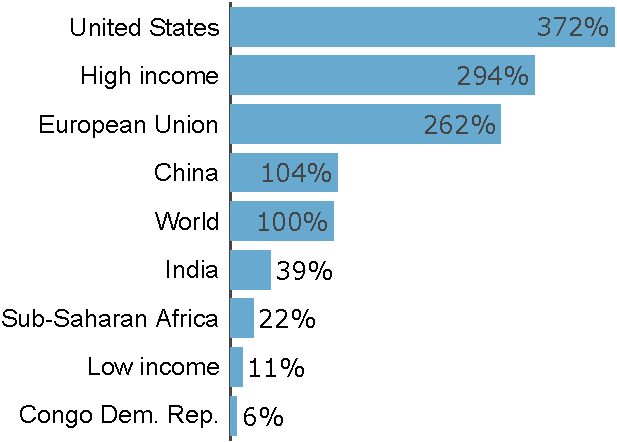
\includegraphics[width=.56\textwidth]{../figures/policies/GDP_pc_PPP_few.pdf}} % https://data.worldbank.org/indicator/NY.GDP.PCAP.PP.CD?contextual=default&end=2021&locations=EU-ZG-XD-XM-1W-IN-US-CD-BI-LU-CN&start=2021&view=bar
\end{figure}

\section{Le lien entre climat et pauvreté}

Quiconque se préoccupe du bien-être des humains veut mettre fin à la pauvreté. 
De mêmee, il n'est pas nécessaire d'attacher une valeur intrinsèque à la Nature ou à la biodiversité pour vouloir lutter contre le changement climatique~; il suffit de se soucier des humains. Le changement climatique met en péril les conditions de vie de larges catégories de population, non seulement dans les générations futures mais aussi contemporaines, en particulier dans les pays tropicaux. En effet, le réchauffement est d'autant plus problématique dans les zones qui sont déjà chaudes --- et abritent l'essentiel des populations pauvres, car ces zones sont davantage exposées à la sécheresse, à la baisse des rendements agricoles, et à la difficulté à travailler en plein air (ou sans climatisation). Non seulement les plus pauvres subissent de plein fouet les effets du changement climatique, mais ils manquent de moyens pour y faire face~: %les populations qui ont à peine de quoi se nourrir
ils n'ont pas les ressources pour acheter un climatisateur, construire une digue ou migrer dans une zone épargnée. 

% Tandis que les principales victimes du changement climatiques sont les générations futures et les populations déjà vulnérables, ce sont les populations les plus aisées qui sont à l'origine des émissions de gaz à effet de serre et ont bénéficié du confort permis par les énergies fossiles. L'enjeu du changement climatique est donc celui d'une injuste répartition des richesses. Pour schématiser, l'opulence d'occidentaux actuels et passés s'est faite au détriment de personnes vulnérables dans les pays du Sud et les générations futures. 

Le changement climatique soulève la question de la répartition mondiale et temporelle du pouvoir, de la richesse, des opportunités et des capacités. En effet, la répartition des émissions de gaz à effet de serre est extrêmement inégale~: alors que les 1~\% d'États-uniens les plus riches émettent en moyenne 318 tCO$_\text{2}$e par an, l'Indien moyen en émet 2 t et les 10~\% les plus pauvres du Honduras ou du Mozambique n'en émettent que 0,1 t\footnote{\citet{chancel_carbon_2015}}. Et contrairement à de nombreux Africains ou Sud-Asiatiques pauvres qui ne sont pas encore nés, les occidentaux riches et âgés à forte empreinte carbone ne souffriront probablement pas tellement du changement climatique et n'ont donc que peu d'intérêt à modifier leur mode de vie opulent\footnote{Comme le montrent les indices de vulnérabilité \citep{chen_university_2015} ou les estimations des dommages du changement climatique en fonction du PIB des pays \citep{burke_global_2015}.}. 
% Reconnaître que les intérêts financiers à court terme de l'élite vont à l'encontre du développement soutenable aide à comprendre que la solution ne viendra probablement pas des dirigeants actuels. 
Ainsi, pour prévenir les impacts dramatiques du changement climatique, il est trompeur de formuler la question simplement en termes de problème environnemental, car le cœur du problème réside dans les inégalités entre les humains qui diffèrent en termes de richesse, d'emplacement ou de génération. En tant que telle, une solution au changement climatique ou à ses impacts ne peut être équitable que si elle implique un transfert substantiel de pouvoir d'achat des riches d'aujourd'hui %(par exemple, par le biais de taxes sur le carbone) 
vers les pauvres de demain.% (par exemple, par le biais de fonds d'adaptation). 

% Une solution au problème couplé des inégalités et du changement climatique nécessitera un élargissement des perspectives. Qui cherche-t-on à favoriser le plus dans ses choix politiques ? Répondre à cette vaste question, en traçant une ligne entre "alliés" et "ennemis", permet de synthétiser l'orientation politique de chacun. On peut classer les gens sur une échelle allant du plus petit au plus grand groupe soutenu : soi-même, ses proches, son ethnie ou sa région, sa nation ou sa religion, tous les humains, l'ensemble de la biosphère. Dans la mesure où nous ne pouvons ressentir de l'empathie, nouer des liens et négocier une solidarité réciproque qu'avec ceux avec qui nous interagissons, il est compréhensible que les humains aient historiquement évolué en clans luttant les uns contre les autres pour le contrôle des ressources. Cependant, pour parvenir à une prospérité harmonieuse, nous devrions nous unir dans un groupe universel de solidarité et lutter ensemble contre des ennemis extérieurs (maladies, catastrophes climatiques) plutôt que contre des personnes avec lesquelles nous pourrions discuter et résoudre pacifiquement nos conflits. Grâce à Internet, il est désormais possible de tisser un réseau de liens interpersonnels nécessaires à la construction d'une société sûre et durable. De plus, l'instauration de la confiance entre les personnes est susceptible de produire des effets positifs importants sur la société, tels qu'une meilleure santé et une réduction des inégalités [Elgar2010] À une époque où les tendances nationalistes et égoïstes gagnent du terrain, il est donc crucial que les humains élargissent leur communauté de solidarité et pensent à long terme. Ce type de pragmatisme doit devenir dominant dans un avenir proche pour que l'opinion générale, les dirigeants et les institutions favorisent équitablement tous les humains (y compris les générations futures) au lieu de défendre les intérêts financiers à court terme de leurs proches ou de leur nation. Un tel humanisme est crucial pour le sort des personnes faibles et du climat. De plus, comprendre que tous les destins sont interdépendants et que le bonheur de chacun dépend des perspectives de bien-être accordées à quiconque[pickett_income_2015] est la seule spiritualité dont la diffusion peut permettre un bonheur durable au plus grand nombre, en projetant un avenir désirable (au lieu de prédire un avenir déprimant). Pour ces raisons, la solution au changement climatique réside davantage dans la bataille d'idées entre humanistes et individualistes que dans le marchandage diplomatique entre pays. 

\chapter{La nécessité de redistribution mondiale\label{ch:redistribution_necessaire}}

Qu'elle soit religieuse, philosophique ou intuitive, la morale prescrit généralement des transferts des personnes à hauts revenus vers les personnes à bas revenus, et donc des pays à hauts revenus vers les pays à bas revenus. C'est le cas de l'utilitarisme, la théorie éthique de référence utilisée en économie. L'utilitarisme attribue le même poids à chaque personne et justifie ainsi le transfert d'un euro d'une personne riche à une personne pauvre, puisqu'un euro procurera plus de satisfaction à cette dernière. D'après la théorie de la taxation optimale, ce raisonnement est valable tant qu'une augmentation des prélèvements n'incite pas les plus riches à réduire, expatrier ou dissimuler leur activité au point de diminuer les recettes obtenues. Des économistes ont calculé le système fiscal optimal en tenant compte de ces effets. Celui-ci réduirait drastiquement les inégalités entre pays et procurerait un revenu minimum de 250\$ par mois au niveau mondial\footnote{Dans ces calculs, \citet{kopczuk_limitations_2005} se limitent à un taux unique (une \textit{flat tax}) et ne s'autorisent pas un barème progressif. Sans cette restriction, le véritable optimum serait encore plus redistributif.}. La théorie de la taxation optimale ne peut rationaliser la situation actuelle qu'en tordant le cou à la morale. En effet, la quasi-absence de transferts internationaux n'est optimale que si on attribue un poids 2~000 fois plus élevé à un États-unien qu'à un Congolais (ou bien, si on attribue une valeur 100 fois supérieure à l'États-unien et qu'on considère que seul un vingtième de l'argent transféré arrivera à son destinataire, le reste étant détourné par la corruption). %de distordre les poids de sorte que la satisfaction d'un États-unien vaille autant que celle de 2~000 Malgaches. 

Au-delà des considérations éthiques, la redistribution mondiale a des fondements juridiques. En 2015, l'ensemble des pays a adopté les Objectifs de développement durable (ODD), au premier rang duquel se trouve l'élimination de l'extrême pauvreté d'ici à 2030. Or, les pays à bas revenus n'ont pas les ressources domestiques suffisantes pour éliminer l'extrême pauvreté. En effet,  dans les 19 pays les plus pauvres, exproprier tous les revenus à partir de 13\$ par jour ne suffirait pas à financer des transferts suffisants pour faire passer leurs 700 millions d'habitants au-dessus de 2\$ par jour d'ici à 2030. Même en faisant l'hypothèse très optimiste d'une croissance du revenu moyen de 7\% par an d'ici à 2030% (soit le maximum observé dans le monde dans les cinq années qui ont précédé la Covid)
, exproprier tous les revenus au-delà de 7\$ par jour ne suffirait pas à éliminer l'extrême pauvreté dans un pays tel que Madagascar\footnote{Ces calculs sont inspirés de \citet{bolch_arithmetics_2022}, reposent sur les données \textit{Poverty and Inequality Platform} de la Banque mondiale, et sont reproductibles sur \href{https://github.com/bixiou/domestic\_poverty\_eradication/code\_poverty/main.R}{github.com/bixiou/domestic\_poverty\_eradication}.}. En d'autres termes, il est impossible d'atteindre le premier ODD sans transferts internationaux. Et ce, alors que le premier ODD se borne à assurer un revenu à peine suffisant pour ne plus avoir faim. Le transfert nécessaire pour ce premier ODD correspond à 0,1\% du PIB mondial, soit autant que les dépenses de nourriture pour les animaux de compagnie. % 2019 poverty gap = 2.6% of $2.15 / world GDP of 16865 https://data.worldbank.org/indicator/SI.POV.GAPS; https://www.grandviewresearch.com/industry-analysis/pet-food-industry

Pour s'assurer une vie décente, qui garantit l'accès à l'eau, l'assainissement, l'éducation, à un système de santé, à une capacité minimale à se déplacer et socialiser, on estime qu'il faut un revenu d'au moins 7\$ par jour\footnote{Cf. \citet{kikstra_decent_2021}.}. Près de la moitié des humains vit sous ce seuil de pauvreté\footnote{Cf. \href{https://ourworldindata.org/grapher/distribution-of-population-between-different-poverty-thresholds-up-to-30-dollars}{ourworldindata.org}.}. Combler l'écart qui les sépare de ce seuil coûterait 2 à 3\% du PIB mondial\footnote{En parité de pouvoir d'achat, cet écart (le \textit{poverty gap}, qu'on peut traduire par \textit{l'étendue de la pauvreté}) est de 4 billions de dollar et le PIB mondial de 140 billions.}. % https://data.worldbank.org/indicator/SI.POV.UMIC.GP https://data.worldbank.org/indicator/NY.GDP.MKTP.PP.KD
En outre, 500 millions de personnes vivent dans un pays où le PIB par habitant est inférieur à ce seuil, et où il est donc rigoureusement impossible d'assurer une vie décente à chacun en mobilisant les seules ressources domestiques. 

En 1970, les pays industrialisés ont pris l'engagement d'allouer 0,7\% de leur PIB à l'aide publique au développement, dont 0,2\% du PIB pour les pays les moins avancés. Cet engagement, renouvelé en 2005 et 2015, n'a été jamais été tenu\footnote{Plus exactement, seule une poignée de pays respecte son engagement : la Suède, la Norvège, le Danemark, le Luxembourg et le Royaume-Uni.}. % TODO donner le chiffre de l'écart
On estime que l'essentiel des ODD pourraient être atteints si les pays industrialisés respectaient enfin cet engagement\footnote{\citet{sdsn_sdg_2019}.}. Pour atteindre une version maximaliste des ODD (y compris assurer l'accès à une énergie propre) ou un autre objectif ambitieux au regard du statu quo (tel qu'assurer 7\$ par jour à chacun), les pays à hauts revenus devraient transférer davantage de ressources, probablement entre 2 et 6\% de leur PIB. 
% Il va sans dire que pour développer des services de santé, d'éducation, une énergie décarbonée, et plus généralement atteindre l'ensemble des ODD, la solidarité internationale est indispensable. Pour assurer 
% Plus généralement, 12 ODD sur les 17 concernent la pauvreté, les inégalités et le changement climatique. Si les pays à bas revenus n'ont déjà pas les ressources nécessaires pour éliminer l'extrême pauvreté (estimées à 0,1\% du PIB mondial), % 2019 poverty gap = 2.6% of $2.15 / world GDP of 16865 https://data.worldbank.org/indicator/SI.POV.GAPS
% il va sans dire qu'une redistribution internationale est nécessaire pour développer des services de santé, d'éducation, une énergie décarbonée, et plus généralement atteindre l'ensemble des ODD.

De tels transferts seraient colossaux. Mais ils pourraient être intégralement supportés par les millionnaires. En se limitant au millième d'humains les plus riches, qui ont une fortune supérieure à 5 millions d'euros, et en ne taxant que leur fortune au-delà de ce seuil, avec un taux effectif progressant de 1\% pour une fortune de 10 millions d'euros à 10\% pour une fortune de 100 milliards, on récolterait environ 2\% du PIB mondial, et leur fortune ne baisserait même pas (puisque la plupart des milliardaires ont des rendements supérieurs à 10\%). % TODO source
Avec une taxation plus progressive, qui démarrerait à 500~000 euros, avec un taux de 0,25\% pour une fortune d'un million d'euro (soit une taxe de 2~500\euro{} par an), et progressant jusqu'à un taux de 20\% sur les plus grosses fortunes, les recettes pourraient atteindre 6\% du PIB mondial. Si une telle redistribution était mise en place, les classes moyennes seraient largement épargnées. Certes, des emplois seraient détruits dans le secteur du luxe, puisque les plus fortunés consommeraient un peu moins, mais d'autres secteurs seraient portés par le développement des pays du Sud et créeraient des emplois orientés vers la production de biens exportés, notamment dans l'industrie. 

% TODO? Comment distribuer ? Créer système de protection sociale, cf. ILO Kenya.
% Si les pays de l'OCDE tenaient leur promesse d'allouer 0,7\% de leur PIB à l'aide publique au développement, dont 0,2\% du PIB pour les pays les moins avancés, les ODD pourraient être remplis\footnote{Cf. \citet{sdsn_sdg_2019}.}. 
% Flux dans l'autre sens

Enfin, les transferts internationaux sont une condition sine qua none pour que les pays à bas revenus se décarbonent. D'une part, ces pays font face à d'autres priorités que la décarbonation et déploient donc le système énergétique le plus abordable --- reposant souvent sur le charbon. D'autre part, ces pays font valoir --- à juste titre --- qu'ils sont les plus vulnérables au changement climatique et qu'ils n'y ont contribué que marginalement\footnote{L'Afrique et l'Asie du Sud sont responsables de 6\% des émissions de CO$_\text{2}$ cumulées. % https://ourworldindata.org/contributed-most-global-co2
}. Dans les négociations internationales, ces pays annoncent généralement deux objectifs de réductions d'émissions : un objectif inconditionnel peu ambitieux et un objectif ambitieux conditionné à des financements extérieurs. Par exemple, l'Éthiopie s'est engagé à réduire inconditionnellement ses émissions de 14\% en 2030 par rapport à un scénario sans action climatique, et conditionne une réduction de 69\% à un financement de 250 milliards de dollar. % https://www.climatewatchdata.org/custom-compare/overview?section=fairness_and_ambition&targets=NGA-revised_first_ndc%2CETH-revised_first_ndc%2CIDN-

Dans les prochains chapitres, nous proposons un Plan mondial pour mettre fin au changement climatique et à l'extrême pauvreté, impliquant d'importants transferts Nord-Sud, tout en étant acceptable pour les populations des pays du Nord.
% ODA for LDCs: only Luxembourg is above the objective of 0.2% of GNI (SDG 17.2) https://data.worldbank.org/indicator/DC.ODA.TLDC.GN.ZS?locations=US-GR-LU-SE-GB&most_recent_value_desc=true
% 19 pays (570M en 2022, 700M en 2030) ne pourraient pas éradiquer l'extrême pauvreté même en expropriant tous les revenus au-delà de 13$/jour. Pays comme la RDC ne pourrait pas mettre fin à l'extrême pauvreté en 2030, même avec une croissance de 6% et en expropriant tous les revenus au-delà de 7$/jour.

% Addressing global poverty, inequalities and climate change are at the heart of the universally agreed Sustainable Development Goals (SDG). % 12 out of  17
% It has been pointed out that low-income countries generally do not have enough domestic resources to eliminate the poverty gap in the short run.\cite{bolch_arithmetics_2022} % In other words, it would hardly be possible to achieve the first SDG and end extreme poverty by 2030 without international transfers. => Careful, Bolch use a poverty line above the SDG one.



\chapter{Le cœur du Plan mondial pour le climat\label{ch:coeur}}
% Le plan mondial pour le climat : les grands principes (description de la mesure, des trajectoires)

% \section{Le cœur du Plan}

On a vu au chapitre \ref{ch:statu_quo} que l'humanité disposait d'un budget carbone à ne pas dépasser pour maintenir le réchauffement sous une cible donnée. L'accord de Paris établit cette cible. En effet, l'intégralité des pays a signé cet accord en 2015, et visent ainsi à contenir le réchauffement <<~nettement en dessous de 2\textdegree{}C (...) en poursuivant l'action menée pour limiter l'élévation de température à 1,5\textdegree{}C~>>. 

Comment garantir une trajectoire d'émissions conforme à ce budget carbone~? Le plus sûr serait de plafonner les émissions mondiales, avec un plafond annuel qui décroît en conformité avec l'objectif. 

Comment alors allouer les permis d'émissions de CO$_\text{2}$~? Le plus simple % naturel, élémentaire
est d'allouer un même permis d'émissions à chaque humain. 

Faut-il autoriser la revente des permis d'émissions~? Oui, % Passer en FAQ la suite ? TODO paragraphe indigeste, à réécrire
instaurer un marché du carbone est préférable à un système de quota carbone non échangeable pour plusieurs raisons, détaillées dans la FAQ en postface. 
%Déjà, si les permis d'émissions ne sont pas échangeables, cela signifie soit que des centaines millions de personnes (notamment dans les pays du Nord) devraient diviser leurs émissions par deux ou trois du jour au lendemain (les mettant dans l'impossibilité de poursuivre leurs activités), soit qu'on allouerait (dans un premier temps) davantage de permis d'émissions aux personnes qui polluent davantage (ce qui romprait avec le principe d'égalité cher aux défenseurs des quotas non échangeables). A contrario, si les permis sont échangeables, les pollueurs auraient une certaine latitude pour choisir leurs émissions et du temps pour adapter progressivement leurs activités et changer leur équipement, tandis que les personnes avec une faible empreinte carbone pourraient revendre leurs permis d'émissions inutilisés et ainsi gagner du pouvoir d'achat. Ainsi, tant les pollueurs que les frugaux bénéficieraient de la flexibilité permise par le marché. D'ailleurs, le bénéfice potentiel serait tellement important que l'émergence d'un marché noir serait difficile à empêcher dans le cas d'un système de quotas non échangeables. Vous vous dites peut-être qu'un marché du carbone serait immoral ou injuste, car il permettrait aux plus riches de continuer à polluer. Pourtant, un tel système opérerait une redistribution des pollueurs vers les frugaux : ceux-là devant payer pour acheter des permis d'émissions à ceux-ci. En outre, mettre en place un marché du carbone n'empêche pas d'interdire par ailleurs les consommations jugées superflues, telles que les yachts, les jets privés, voire les SUV. Enfin, si on considère injuste que les plus riches soient capables de préserver un mode de vie dispendieux dans un tel système, n'est-ce pas parce qu'on considère l'extrême richesse comme injuste~? Si c'est le cas, autant s'attaquer à la fortune directement, plutôt que de passer par des moyens détournés. En effet, plafonner les émissions de Rupert Murdoch ne l'empêcherait pas d'utiliser son empire médiatique pour minimiser, voire nier le changement climatique. %d'Elon Musk ne l'empêcherait pas d'acheter Twitter et d'en contrôler l'algorithme. 

% Un dernier argument contre le marché est qu'il permettrait des enrichissements illégitimes à cause de la fraude ou la spéculation. 

Le système esquissé ci-dessus semble réguler les \textit{individus}. J'ai fait comme si % TODO c'était pas clair que j'avais fait comme si, on peut virer ce passage
les individus auraient la responsabilité d'acheter ou vendre des permis d'émissions, alors qu'on n'a même pas les données pour mesurer précisément les émissions de quelqu'un. En réalité, on peut obtenir des effets équivalents au système esquissé précédemment avec un fonctionnement bien plus simple, qui régule les \textit{entreprises}~: 

Chaque année, un nombre limité de permis d'émissions est créé, en conformité avec la trajectoire d'émissions qu'on s'est fixée. Ces permis d'émissions sont mis aux enchères auprès des entreprises à la source des émissions de CO$_\text{2}$, et en particulier celles qui extraient % TODO mettent sur le marché ?
du charbon, du pétrole ou du gaz. Ces entreprises doivent se procurer des permis correspondant à leurs émissions. Enfin, les recettes générées par la vente de permis sont redistribuées en un revenu de base égal pour tous les humains. 

D'un point de vue théorique, ce système \textit{corporatif} est équivalent au système individuel précédent. En effet, dans le système corporatif, les entreprises polluantes répercutent le coût des permis d'émissions en hausse de prix, si bien que chaque individu ($i$) fait face à une hausse de dépenses ($\Delta d_i$) égale au prix du carbone ($p$) multiplié par son empreinte carbone ($e_i$)~: % TODO simplifier/virer formule
$$ \text{hausse de dépenses}_i = \Delta d_i = p \times e_i\text{.}$$
Quant aux recettes générées, elles correspondent au produit du prix du carbone par l'ensemble des émissions, de sorte que le revenu de base ($r$) est égal au prix du carbone multiplié par l'empreinte carbone moyenne ($\overline{e} = \frac{1}{N} \sum_{i=1}^N e_i$)~:  
$$ \text{revenu de base} = r = p \times \overline{e}\text{.}$$
Dans le système individuel, les permis d'émissions sont alloués de façon égalitaire aux individus, donc les permis d'émissions d'un individu correspondent à l'empreinte carbone moyenne ($\overline{e}$). Ainsi, si une personne revendait tous ses permis d'émissions (au prix $p$), elle toucherait un montant équivalent au revenu de base. Par ailleurs, cet individu devrait alors acheter des permis pour couvrir ses émissions, pour un montant égal au prix du carbone multiplié par son empreinte ($p \times e_i$). Dans les deux cas, on retombe sur le même calcul. Le gain net pour un individu est égal à~: 
$$\text{gain net}_i = r - \Delta d_i = p \times \left( \overline{e} - e_i \right)\text{.}$$
Le système reposant sur les individus est intéressant d'un point de vue théorique, puisqu'il permet de montrer l'équivalence entre allocation des permis d'émissions et allocation des recettes d'une tarification carbone. En revanche, le système d'enchères aux entreprises est le seul qui soit réaliste à administrer. 

Enfin, notons que ces systèmes fixent une quantité~: le régulateur fixe un quota d'émissions et laisse le marché déterminer le prix du carbone. À l'inverse, on pourrait imaginer une taxe carbone~: le régulateur fixe le prix et laisse le marché déterminer les émissions. Pour peu que le prix du carbone soit le même dans le système qui fixe la quantité et celui qui fixe le prix, les deux systèmes sont strictement équivalents (ils entraînent les mêmes émissions tarifées au même prix). Notre proposition repose sur un système qui fixe la quantité puisque l'objectif premier est de respecter le budget carbone (or, fixer le prix ne permet pas de prévoir précisément les émissions). Certes, le système proposé ne permet pas de prévoir précisément le prix du carbone, et un prix trop élevé serait problématique (car il entraînerait des coûts importants pour ajuster nos modes de vie). Mais le prix du carbone peut-être réduit grâce à des mesures complémentaires (cf. chapitre \ref{ch:premier_pas}), et il semble préférable de ne pas sacrifier l'ambition climatique. Cependant, on pourrait fixer le prix sans sacrifier l'ambition à l'aide d'une taxe carbone dont le montant serait révisé annuellement pour s'assurer que la trajectoire d'émissions soit conforme au le budget carbone. Une telle taxe (dont on ne connaît pas précisément le montant plusieurs années à l'avance) serait équivalente au quota que nous proposons. Ainsi, elle constituerait une variante tout à fait valable au Plan proposé, que je soutiendrais tout autant, la différence entre les deux relevant du détail. 

Pour résumer, on peut mettre fin au réchauffement climatique en plafonnant les émissions et éliminer l'extrême pauvreté à l'aide d'un revenu de base. Un système simple et efficace pour traiter ces deux problèmes est de combiner ces deux solutions. Voici le cœur du Plan mondial pour le climat, % TODO changer cette fin?
qui constituent les deux premiers principes détaillés au prochain chapitre. Pour des considérations de justice et de géopolitique, quelques ajustements sont nécessaires pour compléter notre proposition : je les décris ci-après aux principes 3 et 4. Enfin, ce Plan mondial pour le climat doit être complémenté par d'autres mesures~: je les esquisse au chapitre \ref{ch:premier_pas}.


\chapter{Les grands principes du Plan mondial pour le climat\label{ch:principes}}

La proposition développée dans les prochains chapitres ne résout pas tous les problèmes de l'humanité, et ne constitue pas non plus une réponse complète au changement climatique. Bien qu'elle soit désignée <<~Plan mondial pour le climat~>> (parce que ça sonne bien), <<~Cadre international de sortie des énergies fossiles~>> aurait été plus fidèle.  % Une désignation telle que <<~Cadre international de sortie des énergies fossiles~>> aurait été plus fidèle, mais il faut dire que <<~Plan mondial pour le climat~>> sonne mieux. %C'est donc peut-être exagéré de le nommer <<~Plan mondial pour le climat~>>, mais ça sonne mieux qu'une désignation plus fidèle telle que <<~Cadre international de sortie des énergies fossiles~>>. 
En effet, en l'état actuel ce plan couvre uniquement les émissions de CO$_\text{2}$ fossiles et industrielles, pas celles liées à l'usage des terres, à la forêt ou aux autres gaz à effet de serre. % TODO? Inclure toutes émissions ?
Sa portée se limite à établir un traité-cadre qui garantit les réductions d'émissions et détermine les transferts internationaux. Charge ensuite à chaque État ou collectivité de prendre les mesures (climatiques et sociales) appropriées pour que la décarbonation se passe bien sur son territoire. Cette limitation étant posée, examinons les grands principes du Plan.

\section{1$^\text{er}$ principe~: Un quota annuel d'émissions}

Le budget carbone --- et avec lui le climat futur --- est l'élément décisif que les États devront négocier. Dans ce livre, nous interprétons l'accord de Paris comme permettant un dépassement temporaire de la cible de 1,5\textdegree{}C dès lors que le réchauffement n'excède pas 2\textdegree{}C. En d'autres termes, des émissions négatives nettes (à partir de la deuxième moitié de ce siècle) permettront de redescendre jusqu'à 1,5\textdegree{}C, seuil qui sera très probablement déjà franchi en 2040\footnote{\citet{diffenbaugh_data-driven_2023} estiment que le réchauffement dépassera 1,5\textdegree{}C en 2035 dans un scénario de décarbonation ambitieuse, ce qui est cohérent avec la Table 4.2 du rapport de l'\citet{ipcc_climate_2021}.}. 

Notre proposition repose sur un budget d'émissions nettes et couvre la période où les émissions nettes sont positives, c'est-à-dire où les émissions excèdent la séquestration. Pour fixer les idées, disons que le budget d'émissions positives serait de 1~000 GtCO$_\text{2}$ à partir de 2025. Ce budget carbone est conforme à l'objectif de ne pas dépasser les 2\textdegree{}C de réchauffement\footnote{Plus précisément, il y a deux chances sur trois de ne pas dépasser les 2\textdegree{}C de réchauffement avec un budget carbone de 1~000 GtCO$_\text{2}$ à partir de 2024.}. Dans la période suivante, où les émissions nettes seront négatives, il y aurait deux budgets carbone annuels~: un quota d'émissions positives résiduelles (pour les activités impossibles à décarboner), et une commande d'émissions négatives. Un appel d'offre annuel permettrait d'acheter ces émissions négatives au moindre coût, et cette séquestration du carbone serait financée par des taxes sur les plus riches, telles qu'un impôt mondial sur la fortune. Au bout de quelques décennies d'émissions nettes négatives, on atteindra la cible climatique de l'accord de Paris (1,5\textdegree{}C de réchauffement), et on pourrait même continuer de séquestrer du carbone pour atteindre un climat plus clément et limiter la hausse du niveau de la mer. Pour l'instant, ne nous préoccupons pas des émissions négatives, qui ne prendront leur essor que dans quelques décennies, et concentrons-nous sur la première période. 
% Notre proposition repose sur différents budgets carbone~: un budget d'émissions positives, conforme à l'objectif de ne pas dépasser les 2\textdegree{}C de réchauffement, et un budget d'émissions négatives, permettant de réduire la température. Pour fixer les idées, disons que le budget d'émissions positives serait de 1~000 GtCO$_\text{2}$ à partir de 2025, et le budget d'émissions négatives serait de 500 GtCO$_\text{2}$, ce qui signifie que le budget d'émissions nettes serait de $1~000-500=500$ GtCO$_\text{2}$. Pour l'instant, ne nous préoccupons pas des émissions négatives, qui ne prendront leur essor quand dans quelques décennies. 
% Faire différemment pour gérer le plastique : budget carbone jusqu'à net zéro, puis double budget (positif et négatif)
% Pb du plastique: si on le fait payer à l'extraction, on a intérêt à extraire, stocker sous forme de plastiques, et brûler plus tard quand la tonne est plus chère. Comment faire ?

L'organe décisionnaire du Plan définit le quota annuel d'émissions (positives), selon une trajectoire conforme au budget carbone. En début d'année, ce quota est mis aux enchères. %sous la forme de permis d'émissions d'une tonne de CO$_\text{2}$. 
Les sociétés assujetties sont les entreprises ``upstream'', c'est-à-dire celles qui mettent sur le marché des hydrocarbures (charbon, pétrole et gaz), ou dont les procédés industriels émettent du CO$_\text{2}$ (production de ciment, d'hydrocarbures, incinérateurs\dots). 
% Les sociétés assujetties sont les entreprises ``upstream'', c'est-à-dire celles qui extraient des hydrocarbures, importent des biens depuis des pays non participants, ou produisent du ciment\footnote{L'assujettissement pourrait s'opérer un peu plus en aval dans la chaîne de valeur (``midstream''), au niveau des dépôts d'hydrocarbures. Cela permettrait de ne pas faire payer la production de plastique, qui n'engendre pas directement des émissions, et de bénéficier de l'administration existante des droits d'accise sur les produits pétroliers.}. 
Chaque société assujettie transmet la quantité de permis qu'elle s'engage à acheter pour chaque niveau de prix. Pour chaque prix possible, on obtient ainsi une quantité agrégée demandée par les sociétés assujetties. Les permis d'émissions sont alors vendus au prix pour lequel la quantité demandée correspond au quota. Les sociétés assujetties et des sociétés financières agréées peuvent ensuite échanger des permis d'émissions sur un marché secondaire. Au bout de quelques années (probablement une ou deux), le prix d'équilibre aura été découvert, de sorte que le prix sur le marché secondaire sera relativement stable et égal à celui des enchères. En fin d'année, les émissions issues des entreprises assujetties sont contrôlées, et celles-ci doivent délivrer des permis correspondant à ces émissions. Des sanctions dissuasives garantissent le bon fonctionnement du système. Par exemple, pour toute tonne de CO$_\text{2}$ non couverte par un permis d'émissions, la société assujettie devrait payer une amende égale à trois fois le prix d'une tonne de CO$_\text{2}$, et devrait toujours délivrer le permis manquant l'année suivante. % TODO réécrire paragraphe

En résumé, un système d'échange de permis d'émission (ETS, pour \textit{emissions trading system}) serait mis en place pour plafonner les émissions de CO$_\text{2}$ au niveau mondial. 
Un tel système a déjà fait ses preuves dans plusieurs pays, dont l'Union Européenne\footnote{L'ETS européen est souvent décrié. Pourtant, il a bel et bien permis de réduire les émissions couvertes (celles de l'industrie et de la production d'électricité) conformément à l'objectif fixé, tandis que les émissions non couvertes (mais qui vont l'être à partir de 2027) ont continué de croître. En réalité, l'ETS européen a été critiqué pour deux (bonnes) raisons. D'une part, l'objectif fixé n'était pas assez ambitieux (c'est ce qui explique le prix très faible jusqu'à une réforme du système en 2019). D'autre part, les permis d'émissions étaient attribués gratuitement aux entreprises polluantes, plutôt que vendus aux enchères. Ces deux écueils sont évités dans le Plan mondial pour le climat.}, la Chine et la Corée du Sud, et est à l'étude dans d'autres comme l'Inde, le Brésil ou le Nigeria. 17\% des émissions mondiales sont déjà couvertes par un ETS. Différents ETS peuvent être fusionnés avec succès, comme l'ont montré la Californie et le Québec \citep{icap_emissions_2023}. 
% Plan en +, pas fusion
% Détails on sait faire, pas besoin d'en parler ici

\section{2$^\text{e}$ principe~: Un revenu de base mondial}

Les recettes du Plan serviraient à financer un revenu de base mondial~: un même transfert à tous les humains de 15 ans ou plus. Nous estimons que le revenu de base s'élèverait à environ 50\euro{} par mois entre 2030 et 2050, % TODO comment?
ce qui suffirait à sortir de l'extrême pauvreté les 700 millions de personnes qui vivent avec moins de 2 dollars par jour. À leur apogée en 2030, les recettes de l'ETS sont estimées à 5\% du PIB mondial. Le Plan entraînerait des transferts internationaux nets d'environ 1\% % 0,9\%
du PIB mondial, le reste des recettes étant reversé dans le pays où elles sont perçues. Les effets distributifs du Plan sont décrits au chapitre \ref{ch:effets_distributifs}. %En utilisant un scénario limitant le réchauffement climatique à 1,8\textdegree{}C, n
Même si les recettes diminueront lorsque la décarbonation sera presque achevée (vers les années 2060), le revenu de base mondial devrait être maintenu grâce à de nouvelles sources de financement (par exemple, un impôt mondial sur les bénéfices des sociétés). Bien que la distribution d'un revenu de base à chaque être humain soit techniquement difficile, différentes options sont disponibles~: soit les outils administratifs existants, soit des smartphones potentiellement connectés à l'internet par satellite (cf. chapitre \ref{ch:details}).

\begin{figure}[h!]
  \caption{Trajectoires estimées des émissions, du prix du carbone et du revenu de base.}\label{fig:trajectory}
  \makebox[\textwidth][c]{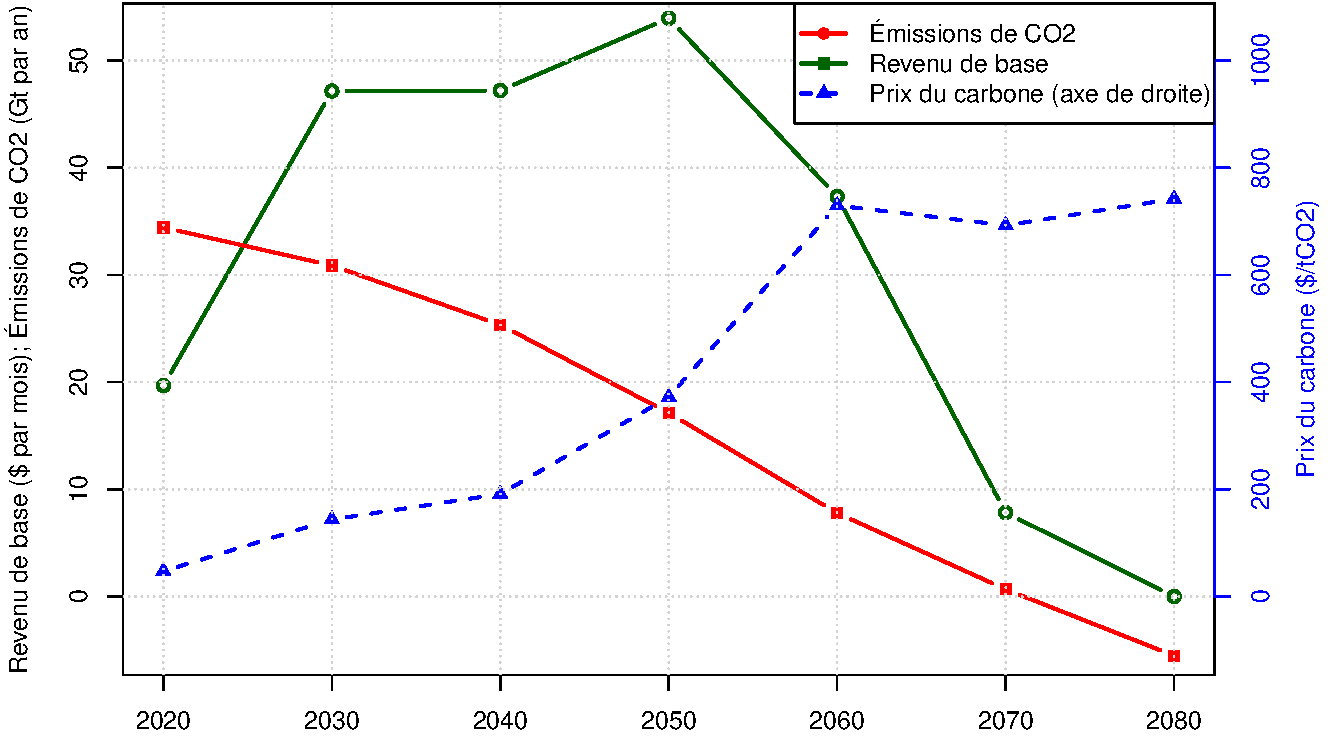
\includegraphics[width=\textwidth]{../figures/policies/GCP_trajectoires.pdf}} 
\end{figure}

\section{3$^\text{e}$ principe~: Un club climatique}

Le Plan serait lancé par un club de pays volontaires et mis en œuvre dès que 60\% des émissions mondiales de CO$_\text{2}$ seraient couvertes par les entités participantes. Ce seuil peut être atteint par l'union de la Chine (30\% des émissions mondiales), des États-Unis (15\%), de l'Inde (7\%), de l'UE et du Royaume-Uni (9\%). Si les États-Unis ne participent pas\footnote{Notons que certains États américains pourraient rejoindre le club même si le niveau fédéral ne le fait pas}, ce seuil serait quand même atteint dans un scénario \textit{Prudent} où le club serait formé par l'UE, les pays qui bénéficieraient financièrement du Plan (23\%, dont l'Inde) et ceux qui ne seraient ni gagnant ni perdant financièrement (35\%, dont la Chine). Dans un scénario \textit{Optimiste} où on ajoute à cela les autres États susceptibles de rejoindre le club\footnote{En plus des pays qui ne seraient pas perdants financièrement et de l'UE, on peut s'attendre à une participation des États suivants~: Royaume-Uni, Japon, Corée du Sud, Norvège, Suisse, Nouvelle-Zélande, Canada, ainsi que les 12 États états-uniens où le parti démocrate a remporté les dernières élections avec plus de 10 points d'écart (en particulier la côte Ouest, l'Illinois, et le Nord-Est à l'exception de la Pennsylvanie).}, 93\% de la population et 76\% des émissions mondiales seraient couvertes (cf. Table \ref{tab:scenarios_table_fr}). 

\begin{table}[h]

\caption[Différents scénarios de club climatique]{\label{tab:scenarios_table_fr}Principales caractéristiques des différents scénarios de club climatique.}
\makebox[\textwidth][c]{
\begin{tabular}[t]{ccccc}
\toprule
\makecell{Scenario\\de club} & \makecell{Émissions\\mondiales\\couvertes} & \makecell{Population\\mondiale\\couverte} & \makecell{Revenu de base\\en 2040\\(\$/mois)} & \makecell{Contribution de l'UE\\en 2040\\(fraction de son PIB)}\\
\midrule
Tous les pays & 100\% & 100\% & 47 & 0.8\%\\
Tous sauf OPEP+ & 90\% & 97\% & 41 & 0.9\%\\
Optimiste & 74\% & 93\% & 32 & 1.1\%\\
Central & 67\% & 90\% & 25 & 1.1\%\\
Prudent & 63\% & 88\% & 22 & 1.2\%\\
UE + Afrique & 12\% & 24\% & 29 & 1.1\%\\
\bottomrule
\end{tabular}}
\end{table}

Les importations vers le club seraient taxées en proportion de leur contenu carbone~: c'est la fameuse tarification carbone aux frontières (que l'UE met en place à son échelle). % TODO virer "fameuse"

\section{4$^\text{e}$ principe~: Des mécanismes de participation}

Une clause dérogatoire (dite d'\textit{opt out}) à la mutualisation des recettes permettrait à des pays (comme la Chine, l'Afrique du Sud ou l'Algérie) dont le PIB par habitant n'excède pas la moyenne mondiale de plus de 50\% de conserver les recettes prélevées sur leur territoire. Cette clause éviterait à des pays aux revenus moyens d'être contributeur net malgré leur empreinte carbone supérieure à la moyenne.
Le traité permettrait également à des États tels que la Californie ou l'État de New York de rejoindre le club indépendamment du niveau fédéral, notamment en les exemptant de la tarification aux frontières.

% 1.	Plafonner les émissions en conformité avec une trajectoire +2°C, à l’aide d’un ETS
% •	Le traité définirait un budget carbone, ensuite décliné en quotas annuels.
% •	Des permis d’émissions de CO2 seraient vendus aux enchères aux entreprises émettrices, comme dans le marché du carbone (ETS) européen.	
% •	Le prix du carbone inciterait les ménages et entreprises à se décarboner. 
% •	Il serait in fine payé par les individus en proportion de leur empreinte carbone.	

% 2.	Utiliser les recettes pour verser un revenu de base mondial et résorber la pauvreté
% •	Les recettes seraient reversées sous la forme d’un revenu de base à tous les adultes.
% •	Chaque humain recevrait ainsi environ 50€/mois.
% •	Les versements sont techniquement possibles (smartphones, internet par satellites). 

% 3.	Former un club climatique avec une tarification carbone aux frontières
% •	Le traité entrerait en vigueur dès que les entités signataires couvrent 60% des émissions mondiales (Chine : 30%, pays bénéficiaires nets : 23%, UE+UK : 9%, U.S. : 15%).
% •	Les importations vers le club seraient taxées en proportion de leur contenu carbone.

% 4.	Inclure des mécanismes qui encouragent la participation de la Chine, la Californie… 
% •	Le traité permettrait à des États de rejoindre l’accord indépendamment du niveau fédéral, notamment en les exemptant de la tarification aux frontières.
% •	Une clause d’opt out de la mutualisation des recettes permettrait à des pays (comme la Chine, l’Afrique du Sud ou l’Algérie) dont le PIB par habitant n’excède pas la moyenne mondiale de plus de 50% de conserver les recettes prélevées sur leur territoire, leur évitant d’être contributeur net malgré leur empreinte carbone supérieure à la moyenne.

% 5.	Complémenter ce Plan par d’autres mesures pour le climat et la justice sociale
% •	Une fiscalité plus progressive pour compenser les classes moyennes des pays riches.
% •	Un ISF mondial finançant les pays pauvres pour traiter les responsabilités historiques.
% •	Des mesures climatiques nationales pour faciliter la décarbonation.


\chapter{Les détails du Plan\label{ch:details}}
% Le plan mondial pour le climat : les détails (implémentation, mécanismes de participation)
% Novissi/Togo: ipa (2021)

\chapter{Un transfert massif vers les pays du Sud\label{ch:effets_distributifs}}
% Le plan mondial pour le climat : les effets distributifs (carte des pays gagnants et perdants)


\begin{figure}[h!]
  \caption{Gains ou pertes financières suite au Plan mondial pour le climat en 2030.}\label{fig:median_gain_2015}
  \centerline{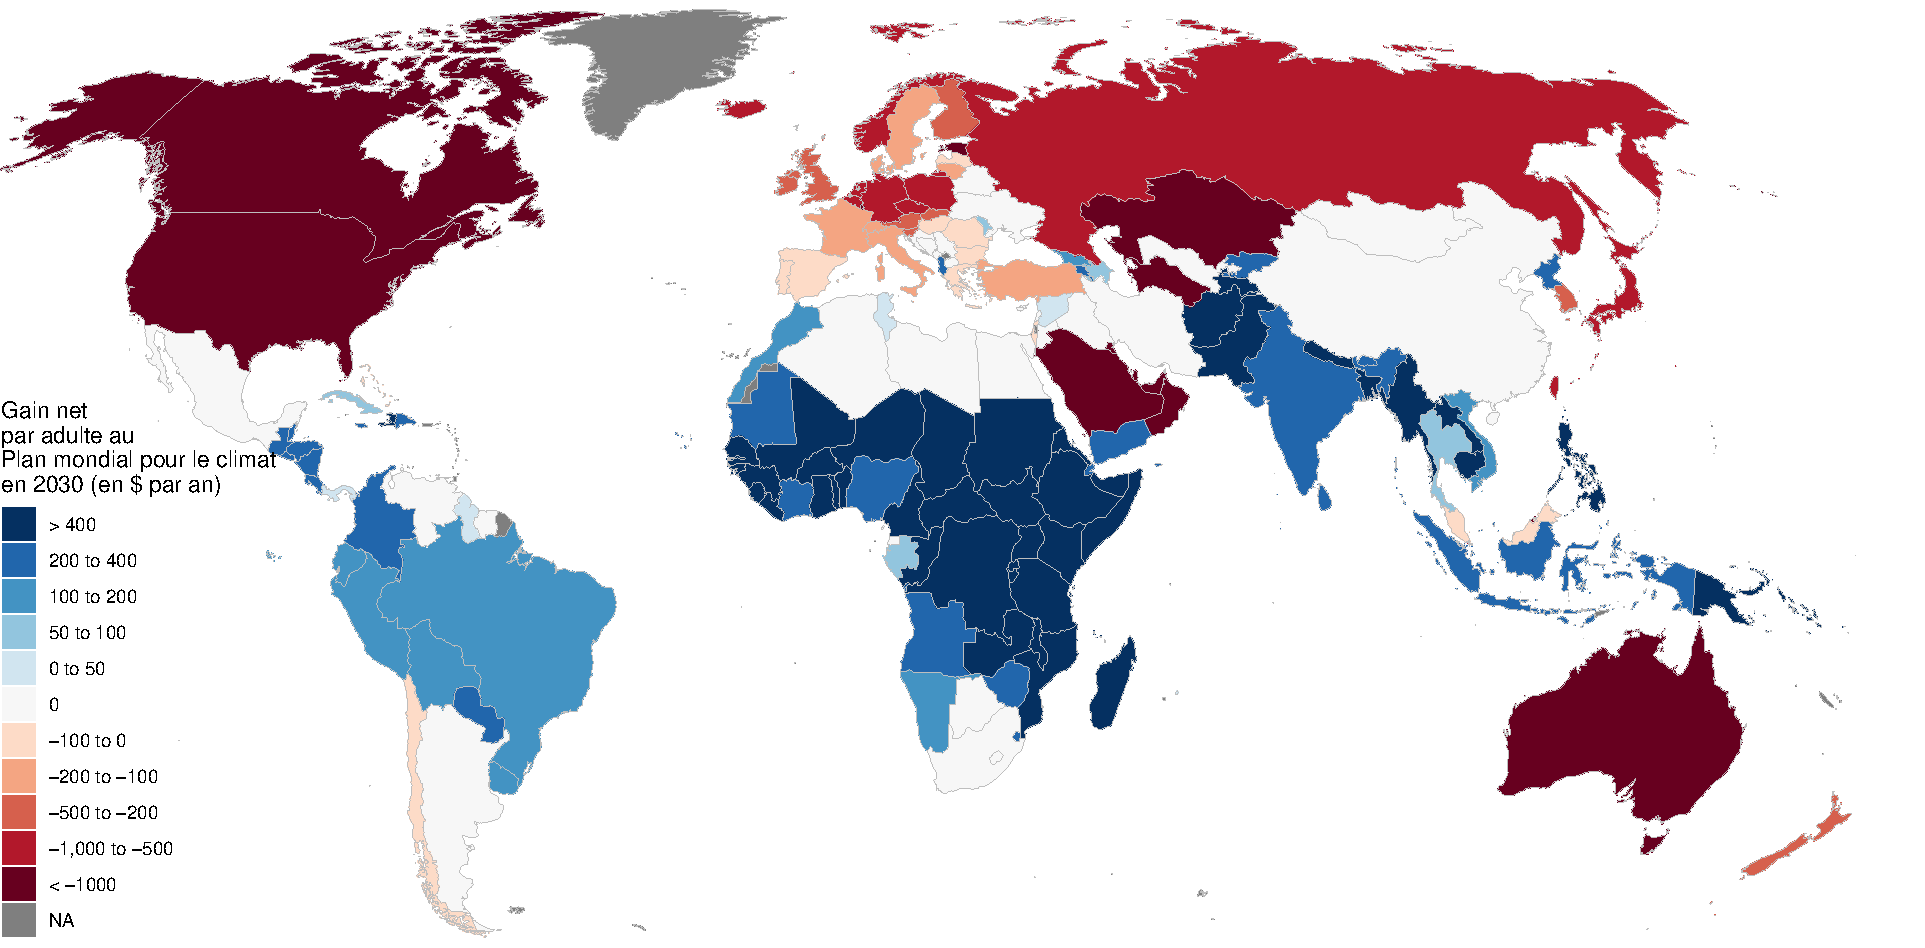
\includegraphics[width=.97\paperwidth]{../figures/maps/gain_adj_2030_fr.pdf}} % mean_gain_over_gdp_2019 mean_gain_2030
\end{figure}

\begin{figure}[b!]
  \caption{Gains ou pertes financières suite au Plan mondial pour le climat sur le XXI$^\text{e}$ siècle}\label{fig:median_gain_adj}
  \centerline{
    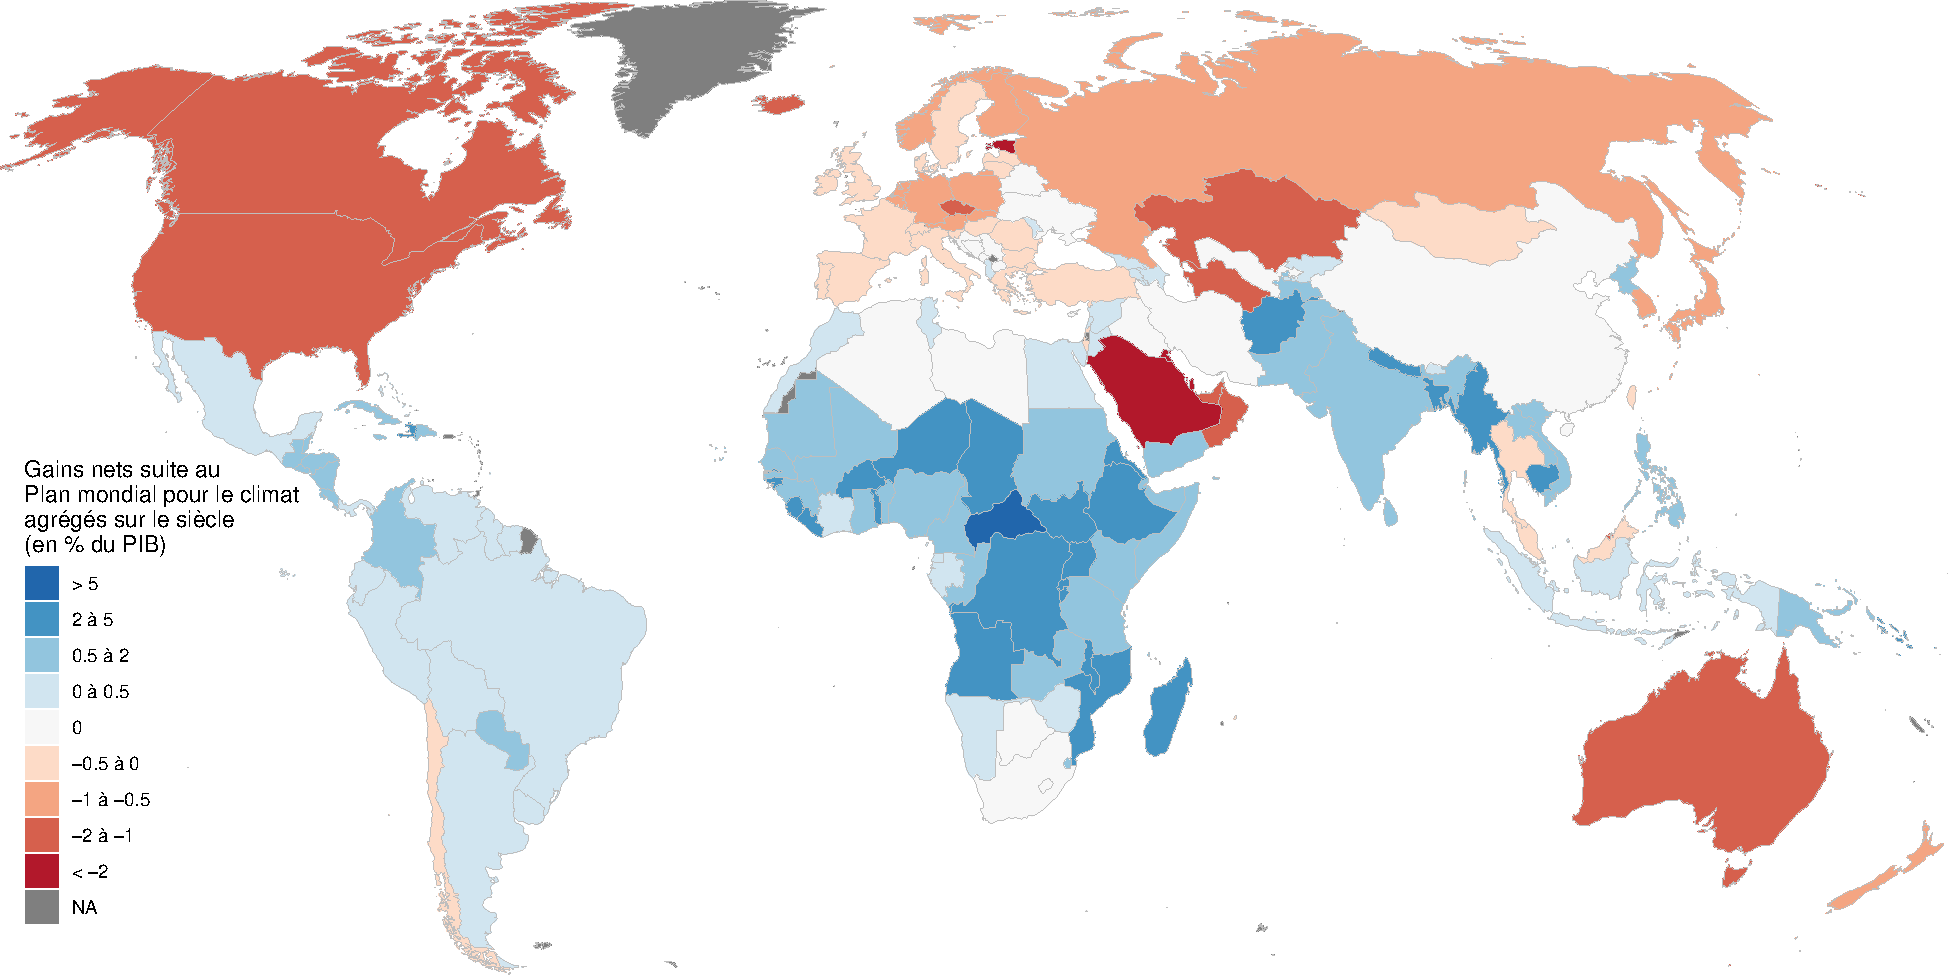
\includegraphics[width=\paperwidth]{../figures/maps/npv_over_gdp_gcs_adj_fr.pdf}
    } % mean_gain_over_gdp_2019
  {\footnotesize \textit{Note:} La valeur nette actualisée est calculée avec un taux d'actualisation de 4\% sur la période 2020 -- 2100.}
\end{figure}

% Une redistribution de 1% de PIB mondial des pays riches vers les pays pauvres.
% •	Le Plan opérerait une redistribution des individus avec une empreinte carbone élevée vers ceux avec une empreinte faible. L’effet serait nul au niveau de la moyenne mondiale.
% •	Lors de leur plateau, entre 2030 et 2050, les recettes correspondraient à environ 5% du PIB mondial, dont 1% en transferts nets entre pays.
% •	Le Français moyen perdrait 14€/mois au pic, soit une perte de 0,4% du revenu national.
% •	Le revenu de base sortirait de l’extrême pauvreté les 700 millions vivant sous les 2$/jour.
% •	Ces estimations ont été faites avec le scénario +2°C central du GIEC, qui implique un prix du carbone d’environ 150$/tCO2 en 2030, 200$ en 2040, 400$ en 2050, et net zéro en 2070.


\chapter{Un Plan largement soutenu\label{ch:soutien}}
% TODO? scinder en deux chapitres et réorganiser?

% Un plan largement soutenu (soutien majoritaire dans 20 pays, avantage électoral aux partis de gauche qui l'incluraient dans leur programme, consensus en faveur de la répartition égalitaire de l'effort de décarbonation)
Ce qui m'a motivé à défendre le Plan mondial pour le climat en montant l'association de plaidoyer \textit{Global Redistribution Advocates} et en écrivant ce livre, c'est le résultat de ma recherche académique. Je me suis spécialisé dans les enquêtes d'opinion relatives au climat et à la redistribution. Ainsi, j'ai mené une enquête internationale dans 20 pays sur les attitudes envers les politiques climatiques, et une enquête complémentaire aux États-Unis et en Europe sur la redistribution mondiale des richesses. Bien que l'idée au cœur du Plan mondial pour le climat --- un quota carbone mondial avec une redistribution égalitaire des recettes --- soit ancienne et considérée comme la politique climatique canonique par les économistes, aucune enquête n'avait testé cette proposition auprès l'opinion publique. Or, les enquêtes révèlent un soutien majoritaire et sincère à travers le monde. C'est cet élément nouveau --- savoir que la population soutient un tel Plan, même dans les pays qui seraient perdants financièrement --- qui justifie de remettre cette idée sur la table des négociations internationales, et qu'on l'étudie sérieusement. Dans ce chapitre, je décrirai l'histoire de cette idée puis les résultats des enquêtes d'opinion.

\section{Une vieille idée} % TODO? mettre au début?
% TODO historique des initiatives alternatives qui vont probablement arriver : debt jubilee, SDG stimulus, Addis-Abeba / Bridgetown initiative, Accra-Marrakech agenda, Hourcade, Paris financial summit + von der Leyen calling for global carbon pricing https://twitter.com/vonderleyen/status/1700416700238225659, vague Fossil Fuel Non-Proliferation treaty (climate movement + Pacific islands + scientists) & fossilfuelfreefuture.org

Le principe du pollueur-payeur est une idée de base en économie, qui remonte à \citet{pigou_economics_1920}. Le principe consiste à faire payer les coûts externes (en l'occurrence, les dégâts causés par le changement climatique) à la personne qui les engendre (ici, l'émetteur de gaz à effet de serre). Cette tarification peut prendre aussi bien la forme d'un marché de quotas que d'une taxe. Le coût qu'elle entraîne pour le pollueur l'encourage à réduire son activité ou la rendre moins polluante, le coût de ces alternatives étant désormais relativement avantageux. Pour neutraliser les coûts externes résiduels, les recettes engendrées devraient servir à prévenir ou remédier aux préjudices causés. Cela dit, dans le cas du changement climatique, les préjudices sont diffus et difficiles à estimer, et il est probablement plus simple de partager les recettes de façon égalitaire. Ce partage égalitaire peut ainsi être conçu comme un égal permis d'émissions pour chaque humain. 

Étant donné ce cadre théorique, il n'est pas étonnant qu'un quota carbone mondial distribué de façon égalitaire soit apparu comme la solution canonique au changement climatique depuis que celui-ci a émergé dans le débat public. Il semblerait que c'est Michael Grubb, professeur à l'University College de Londres, qui a le premier défendu cette solution alors qu'était rédigé le premier rapport du GIEC, en 1990. Dans son article, Grubb écrit que <<~de loin, la meilleure combinaison en termes d'effectivité à long terme, de faisabilité, d'équité et de simplicité est obtenue grâce à un système basé sur des permis d'émission de carbone négociables, attribués sur la base d'un même permis pour chaque adulte~>>\footnote{La citation originale de \citet{grubb_greenhouse_1990} est <<~\textit{by far the best combination of long term effectiveness, feasibility, equity, and simplicity, is obtained from a system based upon tradable permits for carbon emission which are allocated on an adult per capita basis}~>>.}. Un an plus tard, Anil Agarwal et Sunita Narain, du Centre pour la Science et l'Environnement de New Delhi, publient un texte fondateur sur la justice climatique qui défend à peu près la même solution et commence en ces termes~: <<~L'idée selon laquelle les pays en développement tels que l'Inde et la Chine doivent être tenus responsables du réchauffement de la Terre et de la déstabilisation de son climat (\dots) est un excellent exemple de colonialisme environnemental~>>\footnote{La citation originale de \citet{agarwal_global_1991} est <<~The idea that developing countries like India and China must share the blame for heating up the earth and destabilizing its climate, as espoused in a recent study published in the United States (US) by the World Resources Institute (WRI) in collaboration with the United Nations, is an excellent example of environmental colonialism.~>>}. Depuis lors, nombreux sont ceux qui ont témoigné leur soutien à une solution de ce genre~: \citet{bertram_tradeable_1992,baer_equity_2000,jamieson_climate_2001}, ou plus récemment le rapport \citet{blanchard_major_2021}\footnote{Si les auteurs du rapport ne sont pas parfaitement explicites sur la clé de répartition des permis, ils écrivent <<~The European Union should aim at forming a coalition of climate-ambitious countries (including the United States) with a unified ETS market. This climate coalition should encourage other countries to join its ETS in exchange for the distribution of free permits.~>>} (respectivement ancien économiste en chef du FMI et <<~prix Nobel~>> d'économie) et la tribune de \citet{rajan_global_2021} (qui fut gouverneur de la banque centrale indienne et économiste en chef du FMI). 

Hélas, \citet{bertram_tradeable_1992} rapporte que les diplomates de pays riches tels que les États-Unis et le Japon ont évacué cette option des négociations climatiques dès 1990. Au sommet de la Terre de 1992, George Bush exprima clairement que son administration n'était prête à aucune contribution au reste du monde par sa formule restée célèbre~: <<~le mode de vie américain n'est pas négociable~>>. % ``The American way of life is not up for negotiation.'' 
% TODO Le cadre onusien a toujours cherché une solution unanime, avec les US donc. Les négos se sont alors tournées vers politiques nationales dans les seuls pays industrialisés. Kyoto a été un échec à cause de cette scission en deux catégories. On est passé à chercher des réductions d'émissions différenciées contraignantes : échec également (pays du Sud n'étaient pas satisfaits). On est donc passé à des réductions volontaires. 

Dans un livre intitulé <<~Global Carbon Pricing: The Path to Climate Cooperation~>>\footnote{\citet{cramton_global_2017}.}, de nombreux experts, dont trois <<~prix Nobel~>> d'économie (Joseph Stiglitz, Jean Tirole et William Nordhaus), vantent à tour de rôle les mérites d'une tarification mondiale des émissions de CO$_\text{2}$. Dans cet ouvrage, \citet{gollier_negotiating_2015} ordonnent les différentes options possibles pour répartir les recettes de cette tarification selon un paramètre de générosité, et décrivent l'allocation égalitaire des recettes comme étant la plus généreuse envers les plus démunis. % TODO expliquer grandfathering
Dans un autre chapitre, \citet{cramton_international_2015} partent du principe que chaque État défend son intérêt national et proposent l'accord suivant entre les pays %qui veulent agir contre le changement climatique
volontaristes~: Le paramètre de générosité serait choisi par les pays aux émissions par habitant autour de la moyenne mondiale puis l'ambition climatique serait fixée au niveau minimal proposé par les pays participants\footnote{\citet{cramton_international_2015} propose de fixer le prix, mais on pourrait adapter leur proposition à un système d'échange de quotas en fixant le budget carbone, donc je préfère utiliser le terme plus général d'\textit{ambition climatique}.}. Comme les pays aux émissions moyennes sont peu affectés par les transferts internationaux impliqués par l'accord, ils choisiraient stratégiquement le paramètre de générosité qui maximiserait l'ambition climatique~: ni trop élevé, pour que les pays riches proposent un niveau d'ambition importante, ni trop faible, pour que les pays pauvres y gagnent et souscrivent à une ambition importante. \citet{van_den_berg_implications_2020} proposent une ``transition à deux volets vers une tarification mondiale du carbone''~: un club climatique qui fusionnerait les systèmes d'échange de permis existants et en intégrerait progressivement de nouveaux, et une réorientation des négociations internationales (les COP) pour déterminer les règles d'une tarification mondiale du carbone et le niveau de générosité. Le \citet{imf_how_2019} est également favorable à une tarification mondiale du carbone et, dans le court terme, à un prix plancher du carbone. Pour aller dans le sens de la justice climatique, l'institution propose soit des prix différenciés entre les pays, soit la solution que nous défendons~: un prix uniforme avec des transferts internationaux. 

% TODO citer Douthwaite (12) et Kallis et al. (12) qui soutiennent cap & share : des économistes écologistes partisans de la décroissance, et Barnes et al. (08) (dont Ostrom & Costanza) qui défend qu'une fraction (e.g. la moitié) aille en un dividende p.c., le reste pour la mitigation. (C'est la même Barnes qui est à l'origine du Cap & Dividend U.S.)

\section{Une découverte récente~: l'adhésion de la population}

Lors des négociations internationales, les diplomates défendent les intérêts nationaux de court-terme sans se soucier de la justice climatique. Mais représentent-ils correctement leur concitoyens~? % inclusiv
Étonnamment, ce n'est que récemment que des enquêtes d'opinion se sont penchées sur la question. Toutes convergent pour trouver un large soutien en faveur d'une politique climatique mondiale et redistributive. Avant de présenter en détail les résultats d'enquêtes menées par mes collègues et moi-même dans 20 pays et qui examinent le Plan mondial pour le climat, % investiguent, traitent, 
je vais présenter les enquêtes traitant de questions similaires. 
% Si les scientifiques, les responsables politiques et le mouvement associatif se sont pudiquement gardés de défendre un Plan mondial pour le climat jusqu'à présent, c'est peut-être parce qu'il paraît naturel à tout le monde que les diplomates défendent leurs intérêts nationaux de court-terme lors des négociations internationales. Le caractère principalement national des médias, des élections et du pouvoir politique a probablement agi comme des œillères et limité l'élaboration de politiques climatiques à l'échelle nationale.  %e les populations des pays riches n'étaient pas perçues comme prêtes à prendre à sa charge une redistribution mondiale. Comment, si ce n'est par ce présupposé, expliquer que les premières enquêtes à avoir étudié les attitudes envers la justice climatique soient si récentes~? 
% TODO: que défendaient les assos en 90? 95? 00? que défend CAN-I de nos jours?

Depuis une douzaine d'années, une série de travaux académiques s'est attachée à révéler les préférences en termes de la répartition de l'effort de décarbonation entre les pays. Ces études couvrent de nombreux pays à travers des enquêtes toujours représentatives de la population. Si les différentes études sont difficilement comparables car elles diffèrent par leur approche et leur façon de poser les questions, deux régularités se dégagent. Quel que soit le pays dans lequel l'enquête est menée, les options préférées sont celles où l'effort de décarbonation est universel, et celles qui apparaissent égalitaires. %tendent vers l'égalité, évoquent l'égalité, manifestent un souci d'égalité. 
Ainsi, \citet{carlsson_is_2011} trouvent que les Suédois préfèrent qu'il soit permis à tous les pays d'émettre une même quantité d'émissions par habitant. Dans une enquête aux États-Unis, en Allemagne, en France et au Royaume-Uni, \citet{bechtel_mass_2013} révèlent qu'un accord climatique est d'autant plus préféré qu'il comprend un grand nombre de pays, % cf. \citet{beiser-mcgrath_could_2019}
et moins apprécié si les pays riches sont les seuls à porter l'effort de décarbonation par rapport à l'option où <<~les pays riches paient davantage que les pays pauvres~>> ou à celle où les pays <<~paient en proportion de leurs émissions~>>. De même, \citet{carlsson_fair_2013} mettent en évidence que l'option la moins appréciée par les États-uniens ou les Chinois est celle où les pays à faibles émissions sont exemptées de tout effort, tandis que dans une enquête couvrant 28 pays (dont les plus peuplés), une large majorité s'accorde pour que l'intégralité des pays contribue à la réductions des émissions \citep{dabla-norris_public_2023}. \citet{schleich_citizens_2016} rapportent un classement identique des options en Chine, aux États-Unis et en Allemagne, avec une préférence pour le principe du pollueur-payeur suivie par la prise en compte de la capacité à payer, et la dernière place pour l'option où les pays qui polluent le plus ont plus de permis de polluer. Les auteurs trouvent aussi que seuls 13 à 28~\% des gens (suivant les pays) considèrent leur position personnelle correctement représentée dans les négociations internationales~; et 73 à 87~\% pensent que la lutte contre le changement climatique nécessite de nouveaux traités internationaux. Enfin, \citet{meilland_international_2023} trouvent que le principe préféré par les Français et les États-uniens est que <<~tous les pays s'engagent à converger vers une même moyenne d'émissions par habitant, compatible avec un changement climatique maîtrisé~>>.

Dans une enquête de grande ampleur sur 125 pays couvrant 94~\% de la population mondiale, \citet{andre_actual_2024} trouvent que 89~\% des humains souhaitent une politique climatique plus ambitieuse, et 69~\% sont disposés à contribuer 1~\% de leurs revenus pour lutter contre le changement climatique (valeur qui est une estimation crédible du coût de la décarbonation). En revanche, XXX~\% sous-estiment la part de la population disposée à contribuer~: cette part est perçue en moyenne à 43~\%, soit 26 points de moins que la réalité. Cette sous-estimation (dite \textit{ignorance pluraliste}) des préoccupations écologistes explique peut-être le manque d'ambition des accords internationaux sur le climat. 

Alors que les travaux précédents ont investigué des questions d'ordre général ou théorique, très peu d'études ont testé l'adhésion à des mesures climatiques mondiales bien définies. En fait, en dehors de mes propres études, je n'en connais qu'une, publiée dans la revue scientifique \textit{Nature}. Dans cette enquête sur cinq pays, \citet{carattini_how_2019} testent différentes variantes d'une taxe carbone mondiale. Pour la variante avec redistribution égalitaire des recettes, ils trouvent un soutien proche de 50~\% dans les pays à hauts revenus (États-Unis, Australie, Royaume-Uni) et en Afrique du Sud, et plus de 80~\% de soutien en Inde. Ces résultats sont cohérents avec ceux des enquêtes auxquelles j'ai collaborées, détaillés dans \citet{fabre_global_2023}. 

La première de ces enquêtes a été réalisée avec le soutien de l'OCDE entre 2021 et 2022. Avec mes co-auteurs Antoine Dechezleprêtre, Tobias Kruse, Bluebery Planterose, Ana Sanchez-Chico et Stefanie Stantcheva, nous avons conduit une enquête sur les attitudes envers le changement climatique et les politiques climatiques. Cette enquête porte sur 20 pays couvrant 72~\% des émissions mondiales de CO$_\text{2}$ (plus ou moins les pays du G20), avec des échantillons représentatifs d'environ 2~000 répondants par pays. Elle avait pour but principal d'étudier les attitudes envers des politiques climatiques nationales, mais nous avons également posé quelques questions sur des mesures mondiales. Il s'est avéré que parmi les mesures les plus soutenues figurent trois mesures mondiales ayant chacune une forte dimension redistributive~: un quota de permis d'émissions échangeables, une assemblée mondiale élue démocratiquement qui proposerait un traité sur le climat, et un impôt mondial sur la fortune finançant les pays à bas revenus qui respectent les objectifs climatiques. Dans chaque pays, chacune de ces mesures obtient plus de 70~\% de soutien relatif (c'est-à-dire en excluant les réponses \textit{Indifférent\textperiodcentered{}e}), comme le montre la Figure \ref{fig:oecd}. Ces résultats sont cohérents avec une autre question où on demandait à quelle(s) échelle(s) des politiques climatiques sont requises~: % TODO choix multiple
l'écrasante majorité a répondu l'échelle mondiale, tandis que l'échelle continentale ou nationale n'a été choisie que par une petite moitié des répondants. La question sur le quota mondial ne précisait pas l'allocation des permis d'émissions entre pays, mais la question suivante testait le soutien à cette mesure selon différentes variantes pour l'allocation des permis. En cohérence avec les préférences sur la répartition de l'effort révélées par les travaux sus-mentionnés, notre enquête met en évidence un consensus en faveur d'une allocation des permis au pro rata de la population des pays, ce qui correspond à la répartition égalitaire au cœur du Plan mondial pour le climat\footnote{En fait, c'est précisément suite à ce consensus que j'ai défini le Plan sur cette base égalitaire. Si ça ne tenait qu'à moi, j'aurais préféré une approche encore plus redistributive que l'égalitaire.}. Cette variante obtient entre 84~\% et 96~\% de soutien relatif selon les pays, et une majorité absolue de soutien dans tous les pays (même en incluant les réponses \textit{Indifférent\textperiodcentered{}e}). La variante la moins appréciée (mais qui récolte quand même un soutien majoritaire dans la plupart des pays) attribue les permis d'émissions en proportion des émissions actuelles, et n'implique ainsi aucune redistribution Nord--Sud. Un niveau de soutien intermédiaire (qui reste donc élevé) est obtenu par les variantes encore plus redistributives que l'option égalitaire~: celle tenant compte des responsabilités historiques en attribuant moins de permis aux pays qui ont plus émis par le passé, ou celle tenant de la vulnérabilité face au changement climatique en attribuant plus de permis aux pays qui subiront des préjudices plus importants. 
Malgré le soutien extrêmement fort à un quota mondial égalitaire, une taxe carbone mondiale finançant un revenu de base mondial obtient un soutien bien plus faible, autour de 50~\% dans les pays à hauts revenus. Pourtant, les deux mesures sont équivalentes d'un point de vue économique dès lors que le prix du carbone est le même dans les deux systèmes, comme on l'a vu au chapitre \ref{ch:coeur}. Deux facteurs expliquent cet différence dans le soutien. D'une part, les gens peuvent préférer un quota à une taxe, car dans le cas du quota, il est certain que les émissions seront réduites conformément à l'objectif. D'autre part, lorsque nous avons posé la question sur la taxe carbone, nous avons également informé les répondants du coût de ce système sur leur pouvoir d'achat. Sans une enquête complémentaire, nous ne pouvions pas connaître le taux de soutien au Plan mondial pour le climat (c'est-à-dire au quota égalitaire) lorsque les gens sont informés de la perte de pouvoir d'achat qu'il engendrerait. 

\begin{figure}[h!]
  % TODO traduire
  \caption[Soutien aux politiques climatiques mondiales]{Soutien aux politiques climatiques mondiales.} 
  \makebox[\textwidth][c]{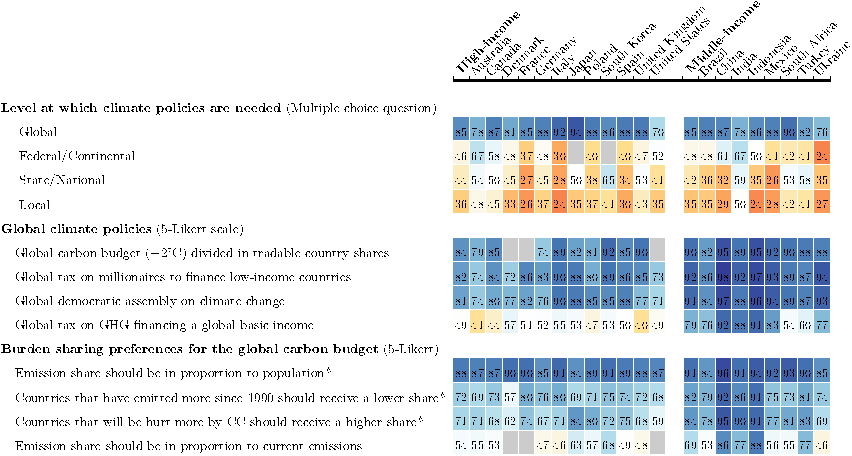
\includegraphics[width=1.2\textwidth]
  {../figures/OECD/Heatplot_global_tax_attitudes_share.pdf}}\label{fig:oecd} % with dependence on others (absent from OECD): Heatplot_burden_share_all_share_countries
  {\footnotesize \\ $\quad$ \\ Note 1: Pourcentage de réponses \textit{Très} et \textit{Plutôt favorable}, en excluant les réponses \textit{Indifférent\textperiodcentered{}e} ($n$ = 40,680). Source~: \citet{fabre_global_2023}. %The numbers represent the share of \textit{Somewhat} or \textit{Strongly support} among non-\textit{indifferent} answers (in percent, $n$ = 40,680). 
  La couleur bleue dénote une majorité relative. %The color blue denotes a relative majority. See Figure \ref{fig:oecd_absolute} for the absolute support. (Questions \ref{q:scale}-\ref{q:millionaire_tax}. Reproduced from \citealp{dechezlepretre_fighting_2022}, Figure A21.) 
  \\ Note 2: *Au Danemark, en France et aux États-Unis, les questions avec une astérisque furent posées différemment. %In Denmark, France and the U.S., the questions with an asterisk were asked differently, cf. Question \ref{q:burden_sharing_asterisk}. 
  } 
\end{figure}

% De 70~\% (aux États-Unis) à 94~\% (au Japon) des personnes interrogées considèrent le niveau mondial comme l'échelle appropriée pour l'adoption de politiques climatiques. En revanche, le niveau européen est choisi par moins de la moitié des répondants européens, le niveau fédéral n'est choisi que par 52~\% des répondants américains, et les niveaux nationaux ou locaux sont choisis par un nombre encore plus restreint de personnes. Il n'est donc pas surprenant que 50~\% (au Japon) à 78~\% (en Chine et en Inde) %74~\% (en Allemagne) à 95~\% (en Chine et en Indonésie) 
% soutiennent le principe d'un système mondial d'échange de permis d'émission. 
% Il est intéressant de noter qu'avec un soutien d'au moins 84~\% dans chaque pays, avec un soutien absolu de 53~\% (au Japon) à 76~\% (en Chine), il existe un consensus mondial en faveur d'un système mondial d'échange de quotas d'émission qui attribue des permis d'émission proportionnellement à la population des pays, conformément à un droit d'émission égal pour chaque être humain. Dans tous les pays, cette solution est préférée à d'autres solutions, telles que l'octroi de droits d'émission supplémentaires aux pays qui ont moins émis dans le passé (\textit{responsabilités historiques}, deuxième option préférée dans l'ensemble), ou aux pays qui émettent actuellement plus (\textit{grandfathering}, option la moins préférée dans l'ensemble). 

Pour comprendre en profondeur les attitudes envers le Plan mondial pour le climat, j'ai mené en 2023 une enquête complémentaire avec deux nouveaux co-auteurs~: Thomas Douenne et Linus Mattauch. Cette enquête repose sur un échantillon représentatif de 3~000 européens (en Allemagne, en Espagne, en France et au Royaume-Uni) et deux échantillons représentatifs de (respectivement) 3~000 et 2~000 états-uniens. 
% \begin{figure}[h !] 
%     \caption{Soutien au Plan mondial pour le climat à travers le monde (en pourcentage).}\label{fig:support}
%     \makebox[\textwidth][c]{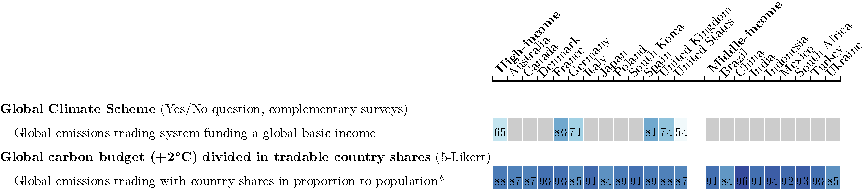
\includegraphics[width=1.2\textwidth]{../figures/OECD/Heatplot_global_tax_attitudes_only_GCS_share.pdf}} 
%     % \makebox[\textwidth][c]{\includegraphics[width=1.2\textwidth]{../figures/OECD/Heatplot_global_tax_attitudes_GCP_share.pdf}} 
% \end{figure}

Voici comment nous avons décrit la mesure aux répondants~:

\begin{quote}
En 2015, tous les pays se sont mis d'accord pour contenir le réchauffement climatique ``bien en-dessous de +2~\textdegree{}C''. Pour limiter le réchauffement climatique à ce niveau, \textbf{il existe une quantité maximale de gaz à effet de serre que nous pouvons émettre à l'échelle mondiale}. \\
Pour respecter cet objectif climatique, on peut créer des permis d'émission de gaz à effet de serre en nombre limité à l'échelle mondiale. Les entreprises polluantes seraient tenues d'acheter des permis pour couvrir leurs émissions. Une telle politique \textbf{obligerait les compagnies pétrolières à payer} leurs émissions et augmenterait progressivement le prix des combustibles fossiles. \textbf{Des prix plus élevés encourageraient les ménages et les entreprises à utiliser moins de combustibles fossiles, réduisant ainsi les émissions de gaz à effet de serre.} \\
Conformément au principe selon lequel chaque être humain a un droit égal à polluer, les revenus générés par la vente de permis pourraient financer un revenu de base mondial. \textbf{Chaque adulte recevrait 30\euro{} par mois}, sortant ainsi de l'extrême pauvreté les 700 millions de personnes qui gagnent moins de 2\$ par jour. \\
~[\textbf{Le Français}]\textbf{ type perdrait financièrement }[\textbf{10\euro{}}]\textbf{ par mois}\footnote{Ce coût mensuel net médian est ajusté suivant le pays. Il est de 85\$ aux États-Unis, 25\euro{} en Allemagne, 5\euro{} en Espagne et 20£ au Royaume-Uni.} (car il ferait face à [40\euro{}] par mois d'augmentations de prix, ce qui est supérieur aux 30\euro{} qu'il recevrait). \\
La mesure pourrait être mise en place dès que des pays qui totalisent plus de 60~\% des émissions mondiales s'accordent dessus. Les pays qui refuseraient de participer à la mesure pourraient faire face à des sanctions (comme des droits de douane) du reste du monde et seraient exclus du revenu de base.
\end{quote}

Nous nous sommes ensuite assurés que les répondants avaient retenu qui gagnerait ou perdrait suite à cette mesure, etnotamment qu'elle serait coûteuse pour les personnes typiques de leur pays. Pour ce faire, nous avons posé des questions de compréhension, puis affiché la réponse correcte. Enfin, nous avons décrit la mesure à nouveau, de façon plus succincte, avant de demander de tester le soutien à l'aide d'une question Oui/Non. 76~\% des Européens et 54~\% des Américains soutiennent la mesure. En Europe, quel que ce soit le pays ou le positionnement politique du répondant, une large majorité soutient le Plan mondial pour le climat. Aux États-Unis, il y a une forte polarisation~: 74~\% des électeurs de Biden soutiennent le Plan tandis que 74~\% des électeurs de Trump s'y opposent, les abstentionnistes le soutenant à 53~\%. Le soutien est plus important pour le quota que pour une taxe carbone (testée dans l'enquête sur 20 pays), ce qui confirme que la population préfère une mesure dont elle est certaine qu'elle réduira suffisamment les émissions de CO$_\text{2}$. Ces résultats montrent que la plupart des occidentaux sont disposés à perdre quelques dizaines d'euros par mois si cela permet de mettre fin au changement climatique et à l'extrême pauvreté. 
% Pour évaluer la robustesse du soutien public constaté dans les 20 pays, \citet{fabre_international_2023} ont mené des enquêtes complémentaires auprès de 3~000 répondants américains et de 3~000 répondants européens (en France, en Allemagne, en Espagne et au Royaume-Uni). Ils décrivent le Plan en détaillant les effets négatifs sur le pouvoir d'achat des personnes interrogées. Malgré l'emphase sur ses coûts, le Plan obtient toujours un soutien majoritaire de 54~\% aux États-Unis et de 76~\% en Europe. À l'aide d'une technique appelée <<~expérience de liste~>>, ils démontrent en outre que ce soutien est authentique et n'est pas motivé par un éventuel biais de désirabilité sociale. En fait, une majorité de personnes dans chaque pays est prête à signer une pétition en faveur du Plan, sachant que la part des répondants prêts à signer sera transmise au cabinet du chef de l'État. 

\begin{figure}[h!]
  % TODO traduire
  \caption[Soutien au Plan mondial pour le climat]{Soutien au Plan mondial pour le climat (pourcent de ``Oui'').} 
  \makebox[\textwidth][c]{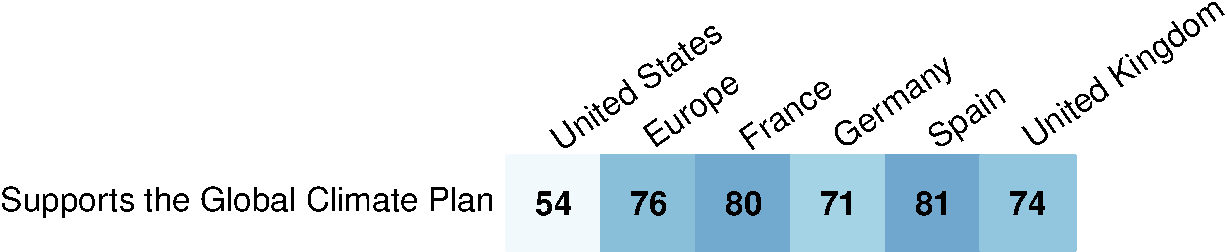
\includegraphics[width=1.2\textwidth]
  {../figures/country_comparison/gcs_support_positive.pdf}}\label{fig:gcs_support} 
\end{figure}

Malgré des réponses très favorables au Plan, on pourrait douter des réponses. Peut-être que les répondants font preuve d'un biais de désirabilité sociale~: ils disent soutenir le Plan car c'est ce qui semble la réponse attendue, les faisant apparaître comme altruistes, même si au fond d'eux ils s'opposent à cette mesure qui nuirait à leur confort et à leur pouvoir d'achat. Peut-être que le résultat serait différent si un référendum avait lieu sur la question (soit que les opinions changent suite au débat médiatique, soit que certaines personnes défendent leur intérêt personnel financier lorsque le choix revêt un véritable enjeu). Peut-être enfin que la plupart des gens soutiennent le Plan mondial pour le climat, mais n'attachent pas à la justice climatique une importance suffisamment importante pour que cette question détermine leur vote aux élections. Par exemple, des personnes qui s'opposent à l'immigration et soutiennent une action climatique ambitieuse pourraient voter pour un parti nationaliste plutôt qu'un parti vert si la question de l'immigration est prioritaire pour elles. La seule façon d'être absolument certains qu'une majorité de la population soutient sincèrement le Plan serait d'organiser un référendum. Mais même à l'aide d'une simple enquête, on peut avoir une bonne indication de la sincérité des réponses, et nous avons utilisé plusieurs méthodes pour la tester dans la suite de l'enquête.

À l'aide d'une technique appelée <<~expérience de liste~>>, nous montrons en outre que le soutien est authentique et n'est pas motivé par un éventuel biais de désirabilité sociale. Cette expérience fonctionne de la façon suivante~: nous demandons aux répondants \textit{combien} de mesures ils soutiennent parmi une liste de mesure. Pour un groupe aléatoire de répondants, la liste contient trois mesures (en Europe, les trois mesures que nous avons employées sont~: la peine de mort pour les crimes majeurs, un plan de redistribution nationale et un plan d'isolation thermique des bâtiments). Pour un autre groupe aléatoire de répondants, la liste contient quatre mesures~: les trois mesures précédentes ainsi que la mesure qui nous intéresse, le Plan mondial pour le climat. Comme on demande seulement aux répondants \textit{combien} de mesures ils soutiennent, on ne sait pas quelles mesures un répondant donné soutient. Pour cette raison, les répondants ne font plus face à un biais de désirabilité sociale les incitant à mentir sur leur soutien à telle ou telle mesure. Par ailleurs, cette méthode permet quand même d'estimer le soutien à la mesure qui nous intéresse, en faisant la différence entre le nombre moyen de mesures soutenues dans le groupe avec la liste à quatre mesures et celui de la liste à trois mesures. Par exemple, si le groupe à trois mesures en soutient en moyenne 2,1, et le groupe à quatre mesures 2,86, on peut faire l'hypothèse que le groupe à quatre mesure soutient autant les trois premières mesures que l'autre groupe (puisqu'ils sont chacuns représentatifs de la population), et que la différence entre le nombre de mesures soutenues correspond au soutien à la quatrième mesure, soit $2,86 - 2,1 = 76~\%$ de soutien tacite en faveur du Plan mondial pour le climat. On peut alors estimer le biais de désirabilité sociale en comparant le soutien tacite au soutien déclaré à la question directe, rapporté précédemment. Dans d'autres contextes, cette méthode a révélé un biais de désirabilité sociale en faveur de l'invasion de l'Ukraine parmi la population russe (le soutien tacite étant 10 à 20 points plus faible que le soutien déclaré), ou encore la sous-déclaration d'opinions racistes dans le Sud des États-Unis\footnote{\citet{kuklinski_racial_1997,chapkovski_solid_2022}}. Dans notre enquête, le soutien tacite n'est pas significativement différent du soutien déclaré, ce qui indique que le soutien est authentique et n'est pas motivé par un éventuel biais de désirabilité sociale. 

Pour approcher du mieux qu'on peut l'enjeu que constituerait un référendum, nous avons demandé aux répondants s'ils sont prêts à signer une pétition en faveur du Plan mondial pour le climat, en sachant que les résultats à cette question (posée à un échantillon représentatif de la population) seront transmis au cabinet du chef d'État. Ainsi, les répondants comprenaient que leur réponse pouvait avoir une influence sur la politique officielle. Aux États-Unis, une majorité est prête à signer la pétition, et la différence avec le soutien déclaré direct n'est pas significative. En Europe, 69~\% des répondants sont prêts à signer la pétition~: c'est certes 7 points de moins que pour le soutien déclaré, mais ça reste une large majorité. 

La preuve la plus convaincante que le soutien au Plan est profond est qu'un candidat progressiste pourrait gagner des voix en le soutenant. Nous le montrons en utilisant différentes questions. Tout d'abord, nous décrivons un programme progressiste et un programme conservateur correspondant aux programmes typiques des principaux partis du pays, nous présentons le choix entre les deux programmes comme étant celui entre les deux candidats de la prochaine élection majeure (en France, le second tour de la prochaine élection présidentielle), et nous demandons aux personnes interrogées pour quel candidat elles voteraient. Pour une moitié aléatoire de l'échantillon, nous ajoutons le Plan mondial pour le climat au programme progressiste. En France, le candidat progressiste gagnerait 11 points de vote en incluant le Plan dans son programme. Aux États-Unis, le candidat progressiste pourrait gagner 3 points, tandis que dans les autres pays, l'effet n'est pas significativement différent de zéro (même au seuil de 20~\%)\footnote{Le gain électoral est très significatif en France (la valeur $p$ est de 0,5~\%). Pour les États-Unis, la valeur $p$ est de 13~\%, c'est-à-dire non statistiquement significative au seuil habituel de 5~\%, mais avec seulement 13~\% de chances que le candidat progressiste n'ait aucun gain électoral en soutenant le Plan. Pour les autres pays, le gain électoral n'est pas significativement différent de zéro.}. Ainsi, le soutien au Plan mondial pour le climat ne ferait perdre des voix à un candidat progressiste dans aucun pays, et pourrait rapporter un gain électoral important en France. 

Dans la question suivante, nous tirons au sort deux programmes politiques à partir d'un ensemble de mesures (plutôt progressistes), puis nous ajoutons le Plan à l'un des programmes. En Europe, les personnes interrogées sont invitées à imaginer qu'une coalition de gauche ou de centre-gauche remportera les prochaines élections et il leur est demandé sur quel programme elles préféreraient que cette coalition ait fait campagne. Aux États-Unis, la question est formulée comme un duel hypothétique dans une primaire démocrate et n'est posée qu'aux non-républicains (c'est-à-dire aux démocrates, aux indépendants et aux non-affiliés). La plate-forme contenant le Plan est systématiquement préférée par une majorité (allant de 58~\% aux États-Unis et au Royaume-Uni à 64~\% en Espagne). Cette question et la précédente révèlent que le soutien au Plan mondial pour le climat est non seulement sincère, mais est aussi suffisamment important pour déterminer le choix électoral de certains électeurs. 

\begin{figure}[h!] % TODO traduire
  \caption[Influence du Plan sur la plateforme préférée]{Influence du Plan sur la plateforme préférée~:\\ Préférence pour une plateforme aléatoire A contenant le Global Climate Scheme plutôt qu'une plateforme B n'en contenant pas (en pourcent). (Aux États-Unis, question posée uniquement aux non-Républicains).}\label{fig:conjoint_left_ag_b}
  \makebox[\textwidth][c]{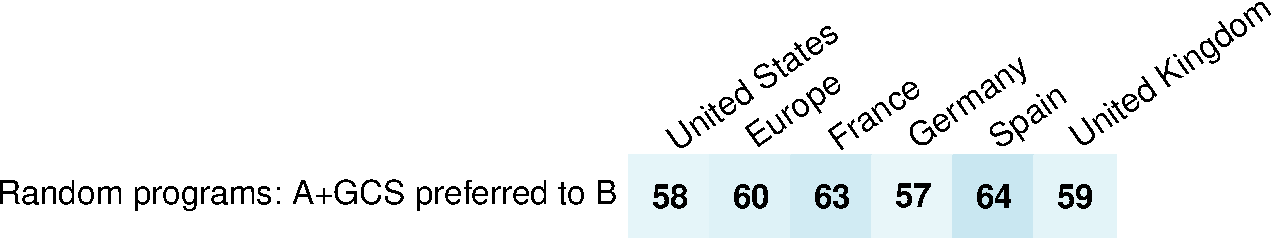
\includegraphics[width=\textwidth]{../figures/country_comparison/conjoint_left_ag_b_binary_positive.pdf}} 
\end{figure}

Enfin, cette priorisation du Plan est confirmée lors d'une question demandant aux répondants de répartir 100 points pour exprimer leur soutien à un ensemble de mesures (le même que précédemment), avec la consigne d'attribuer davantage de points aux mesures qu'ils soutiennent le plus. Le Plan mondial pour le climat est plus priorisé que la moyenne et fait partie des politiques climatiques les plus appréciées. À l'inverse, une mesure climatique promulguée dans l'UE et en Californie (l'élimination progressive des nouvelles voitures à moteur à combustion) est l'une des trois politiques les moins priorisées dans chaque pays. Plus généralement, cette question montre que les mesures de redistribution mondiales sont assez prioritaires pour l'électorat, juste derrière les mesures les plus appréciées~: l'augmentation du salaire minimum et l'amélioration des services publics grâce à des financements supplémentaires pour l'éducation et la santé.

Pour résumer, les enquêtes d'opinion révèlent un soutien majoritaire large et sincère en faveur du Plan mondial pour le climat, et indiquent que la population préfère les programmes politiques qui incluent cette mesure aux programmes qui ne la contiennent pas. Et ce, alors même que les répondants occidentaux sont pleinement conscients qu'ils perdraient un peu de pouvoir d'achat dans le cadre du Plan mondial pour le climat. Pour en savoir plus sur ces enquêtes (lire le questionnaire, les méthodes précises et les résultats complets), je renvoie le lecteur vers l'article académique intitulé \textit{International Attitudes Toward Global Policies}, que j'ai co-écrit avec Thomas Douenne et Linus Mattauch.

\chapter{Un pas vers un monde soutenable\label{ch:premier_pas}}
% Un pas vers un monde soutenable (le Plan n'est pas suffisant, il doit être complémenté d'autres mesures climatiques (nationales, sectorielles), d'autres mesures de redistribution mondiale (impôt sur la fortune), et l'objectif de long terme doit être d'assurer les conditions nécessaires au bien-être à chaque humain)

\chapter{L'appel pour la redistribution mondiale\label{ch:appel}}
% L'appel pour la redistribution mondiale (description de l'activité de Global Redistribution Advocates et de CASCA, lien vers la lettre ouverte aux dirigeants pour la redistribution mondiale - que nous prévoyons de publier dans les grands journaux type The Guardian, Le Monde..., appel à une manifestation mondiale en soutien à cet appel le 1er décembre 2024 lors de la COP29).

\textbf{Nous exhortons les dirigeants mondiaux à mettre en œuvre des politiques de redistribution mondiale~!}

Nous exhortons les dirigeants mondiaux à mettre en œuvre des politiques visant à mettre fin à la pauvreté, à stopper le réchauffement climatique et à réduire les inégalités. 
Pour atteindre le premier objectif de développement durable et mettre fin à l'extrême pauvreté d'ici 2030, des transferts internationaux sont nécessaires. Pour réussir la décarbonisation dans les pays à bas revenus, des transferts internationaux sont nécessaires. Pour permettre à tous les humains de mener une vie décente, des transferts internationaux sont nécessaires. 

L'écart est sidérant entre les niveaux de vie des pays à hauts revenus, où vivent 1,2 milliard de personnes, et ceux des pays à bas revenus, où vivent 700 millions de personnes. Le PIB par habitant est 62 fois plus élevé dans les pays à hauts revenus que dans les pays à bas revenus. En d'autres termes, un transfert de seulement 1~\% du PIB des pays à haut revenus vers les pays à bas revenus doublerait mécaniquement le revenu national de ces derniers. Un transfert de cette ampleur peut être financé par un impôt sur la fortune modéré, de 2~\% sur le patrimoine au-delà de 5 millions de dollars, ce qui laisserait 99,9~\% de la population non affectée.

Dans le monde entier, des majorités écrasantes soutiennent les mesures de redistribution mondiale. Les pays du Sud défendent un ensemble de revendications et de propositions de redistribution mondiale. Il est temps d'agir. Les solutions sont connues~:

Premièrement, il faut un système fiscal viable. Pour lutter contre l'évasion fiscale, les autorités fiscales doivent intensifier leur coopération grâce à l'échange automatique d'informations et à la création d'un registre mondial des actifs, facilitant l'identification de leurs bénéficiaires ultimes. Pour contrecarrer le dumping fiscal, des taux d'imposition minimaux doivent être établis, en particulier sur les bénéfices des entreprises. L'impôt sur les sociétés doit préserver l'intérêt des pays à bas revenus~; en particulier, l'apportionnement des bénéfices d'une société multinationale doit tenir compte de la localisation de ses employés au moins autant que de celle de ses ventes. 

Deuxièmement, il faut un système financier inclusif. L'accès au financement reste un formidable défi pour les pays à bas revenus, accablés par des taux d'intérêt prohibitifs. L'initiative Bridgetown 2.0, proposée par le secrétaire général des Nations unies et la première ministre de la Barbade, offre une série de solutions. Pour <<~dé-risque~>> les projets de développement soutenable, il faut des garanties publiques sur le crédit et le marché des changes. Pour amplifier le financement du développement, les banques multilatérales de développement doivent être recapitalisées et recevoir des Droits de Tirage Spéciaux~; la dette publique des pays à faible revenu doit être restructurée~; et les prêts publics doivent être augmentés pour atteindre 500 milliards de dollars par an. (c'est le stimulus tant attendu pour les objectifs de développement durable). 

Troisièmement, il faut un système fiscal international. Pour atteindre l'objectif climatique universellement adopté dans l'Accord de Paris, nous devrions créer un régime mondial de taxation du carbone, comme le demande l'Union africaine.  À terme, ce régime pourrait prendre la forme d'un système mondial d'échange de quotas d'émission, dont les recettes financeraient un revenu de base mondial. Dans un premier temps, nous devrions introduire des taxes carbone sur le transport maritime et aérien. Il faut également instaurer une taxe sur les transactions financières afin de générer des revenus rapidement, et des impôts sur la fortune pour lutter contre les inégalités. Au moins un tiers des recettes de ces nouvelles taxes devrait être alloué aux pays à bas revenus, en fonction décroissante de leur PIB par habitant.

Quatrièmement, il faut une gouvernance mondiale démocratique. La redistribution mondiale s'applique également à la prise de décision. Pour les décisions qui doivent se prendre à l'échelle mondiale, nous devrions avancer vers une Assemblée parlementaire des Nations unies élue au suffrage direct et dotée d'un pouvoir décisionnaire. À court terme, nous pourrions expérimenter le fédéralisme mondial à travers des assemblées mondiales limitées à un rôle consultatif, qui procèderaient soit d'une élection, soit d'un tirage. Dans tous les cas, les citoyens du monde doivent bénéficier d'une représentation proportionnelle.

Nous appelons les dirigeants mondiaux à examiner des mesures de redistribution mondiale telles que celles décrites ci-dessus lors des réunions de l'ONU, du G20 et des COP. Nous exhortons les décideurs à mettre en œuvre des politiques mondiales redistribuant au moins 1~000 milliards de dollars par an (c'est-à-dire 1~\% du revenu mondial) des pays à hauts revenus vers les pays à bas revenus. Ce ne serait qu'un premier pas vers un monde moins inégalitaire.

Nous sommes un groupe divers d'organisations de la société civile, d'universitaires, de responsables politiques, de syndicats, de groupes religieux, de célébrités et de citoyens du monde. Chacun et chacune est invitée à rejoindre notre mouvement en signant cette lettre ouverte, en diffusant son message, en faisant campagne pour la redistribution mondiale ou en faisant un don à la cause. Nous manifesterons notre force et notre détermination dans un an, le jeudi 17 octobre 2024, à l'occasion de la Journée internationale pour l'élimination de la pauvreté. Inscrivez cette date sur vos calendriers, car elle constituera un moment décisif dans la quête mondiale pour la justice et l'équité.


\chapter{Foire Aux Questions\label{ch:faq}}

% FAQ
% - Les émissions vont augmenter si on distribue un revenu de base et les revenus augmentent
% - Qui paient : entreprises ou consommateurs ?
% - Les quotas profitent aux plus riches qui peuvent s'acheter plus de quotas, les plus pauvres bradent leurs quotas pour des rétributions immédiates en obérant des potentialités pour le futur 
% - pas sûr que ça ait fait ses preuves 
% - il y a certaines pratiques qui vont devoir s'arrêter, il faut interdire
% => Le Plan fournit un cadre qui assure des réductions d'émissions adéquates; qui incite les États à prendre des mesures complémentaires type interdiction; on peut remplacer le système d'échanges de permis par une taxe, c'est équivalent. 
% Pourquoi pas taxe progressive ?
% Problème de la fraude / du monitoring.
% Problème de la transparence sur les implications (les gens réalisent-ils les changements de mode de vie nécessaires ?)
% Qu'est-ce qu'on fait de l'EU ETS? On le laisse en place. 
% Les taxes affectées ne sont-elles pas interdites ? => no, e.g. Chirac tax on flying
% - Est-ce possible d'assurer une vie décente à chacun dans un monde décarboné ?

% \begin{center}
% {\textbf{\href{https://github.com/bixiou/global_tax_attitudes/raw/main/paper/book.pdf}{Link to most recent version}}}
% \end{center}

% 0. Préface : j'envisage Thomas Piketty, Jean Tirole, Gaël Giraud ou Esther Duflo pour la version française et Greta Thunberg ou Joseph Stiglitz pour la version anglaise (mais ça reste à définir)
% 1. Un statu quo insupportable : l'extrême pauvreté, le changement climatique (chiffres, constat)
% 2. La nécessité de redistribution mondiale (objectifs de développement durable, justifications théoriques)
% 3. Le plan mondial pour le climat : les grands principes (description de la mesure, des trajectoires)
% 4. Le plan mondial pour le climat : les détails (implémentation, mécanismes de participation)
% 5. Le plan mondial pour le climat : les effets distributifs (carte des pays gagnants et perdants)
% 6. Un plan largement soutenu (soutien majoritaire dans 20 pays, avantage électoral aux partis de gauche qui l'incluraient dans leur programme, consensus en faveur de la répartition égalitaire de l'effort de décarbonation)
% 7. Un pas vers un monde soutenable (le Plan n'est pas suffisant, il doit être complémenté d'autres mesures climatiques (nationales, sectorielles), d'autres mesures de redistribution mondiale (impôt sur la fortune), et l'objectif de long terme doit être d'assurer les conditions nécessaires au bien-être à chaque humain)
% 8. L'appel pour la redistribution mondiale (description de l'activité de Global Redistribution Advocates, lien vers la lettre ouverte aux dirigeants pour la redistribution mondiale - que nous prévoyons de publier dans les grands journaux type The Guardian, Le Monde..., appel à une manifestation mondiale en soutien à cet appel le 1er décembre 2024 lors de la COP29).
% 9. Postface : Foire Aux Questions (description et réponse aux objections habituelles)

% Un plan mondial pour le climat et contre l'extrême pauvreté (version courte illustrée / version longue) :
% - situation pauvreté, csq CC
% - SDGs, justifications redistr. mondiale
% - description GCS, y.c. trajectoires
% - détails implémentation (e.g. Aadhaar)
% - acceptation
% - autres mesures mondiales possibles
% - appel signé par milliers + manif mondiale un an après lancement
% - préface Piketty puis Greta
% - FAQ, y.c. critiques d'une page (et réponses) de Piketty, etc.
% Opuscule Cepremap au pire

% Wealth tax: 
% taxe universelle ? exit tax ?

\renewcommand{\url}[1]{\href{#1}{Link}} % NCCcomment
\bibliographystyle{plainnaturl_clean} % NCCcomment
\bibliography{global_tax_attitudes}

\end{document}

% L'UE régule midstream: dépôts pétroliers pour l'ETS2 (entre raffinerie et pompe) ou installations pour ETS1. Pourquoi pas upstream? Car on se repose sur l'administration des droits d'accise existante, qui fonctionne bien.